\section{Local Vertex Colouring}
% \begin{figure}[ht]
% \centering
% 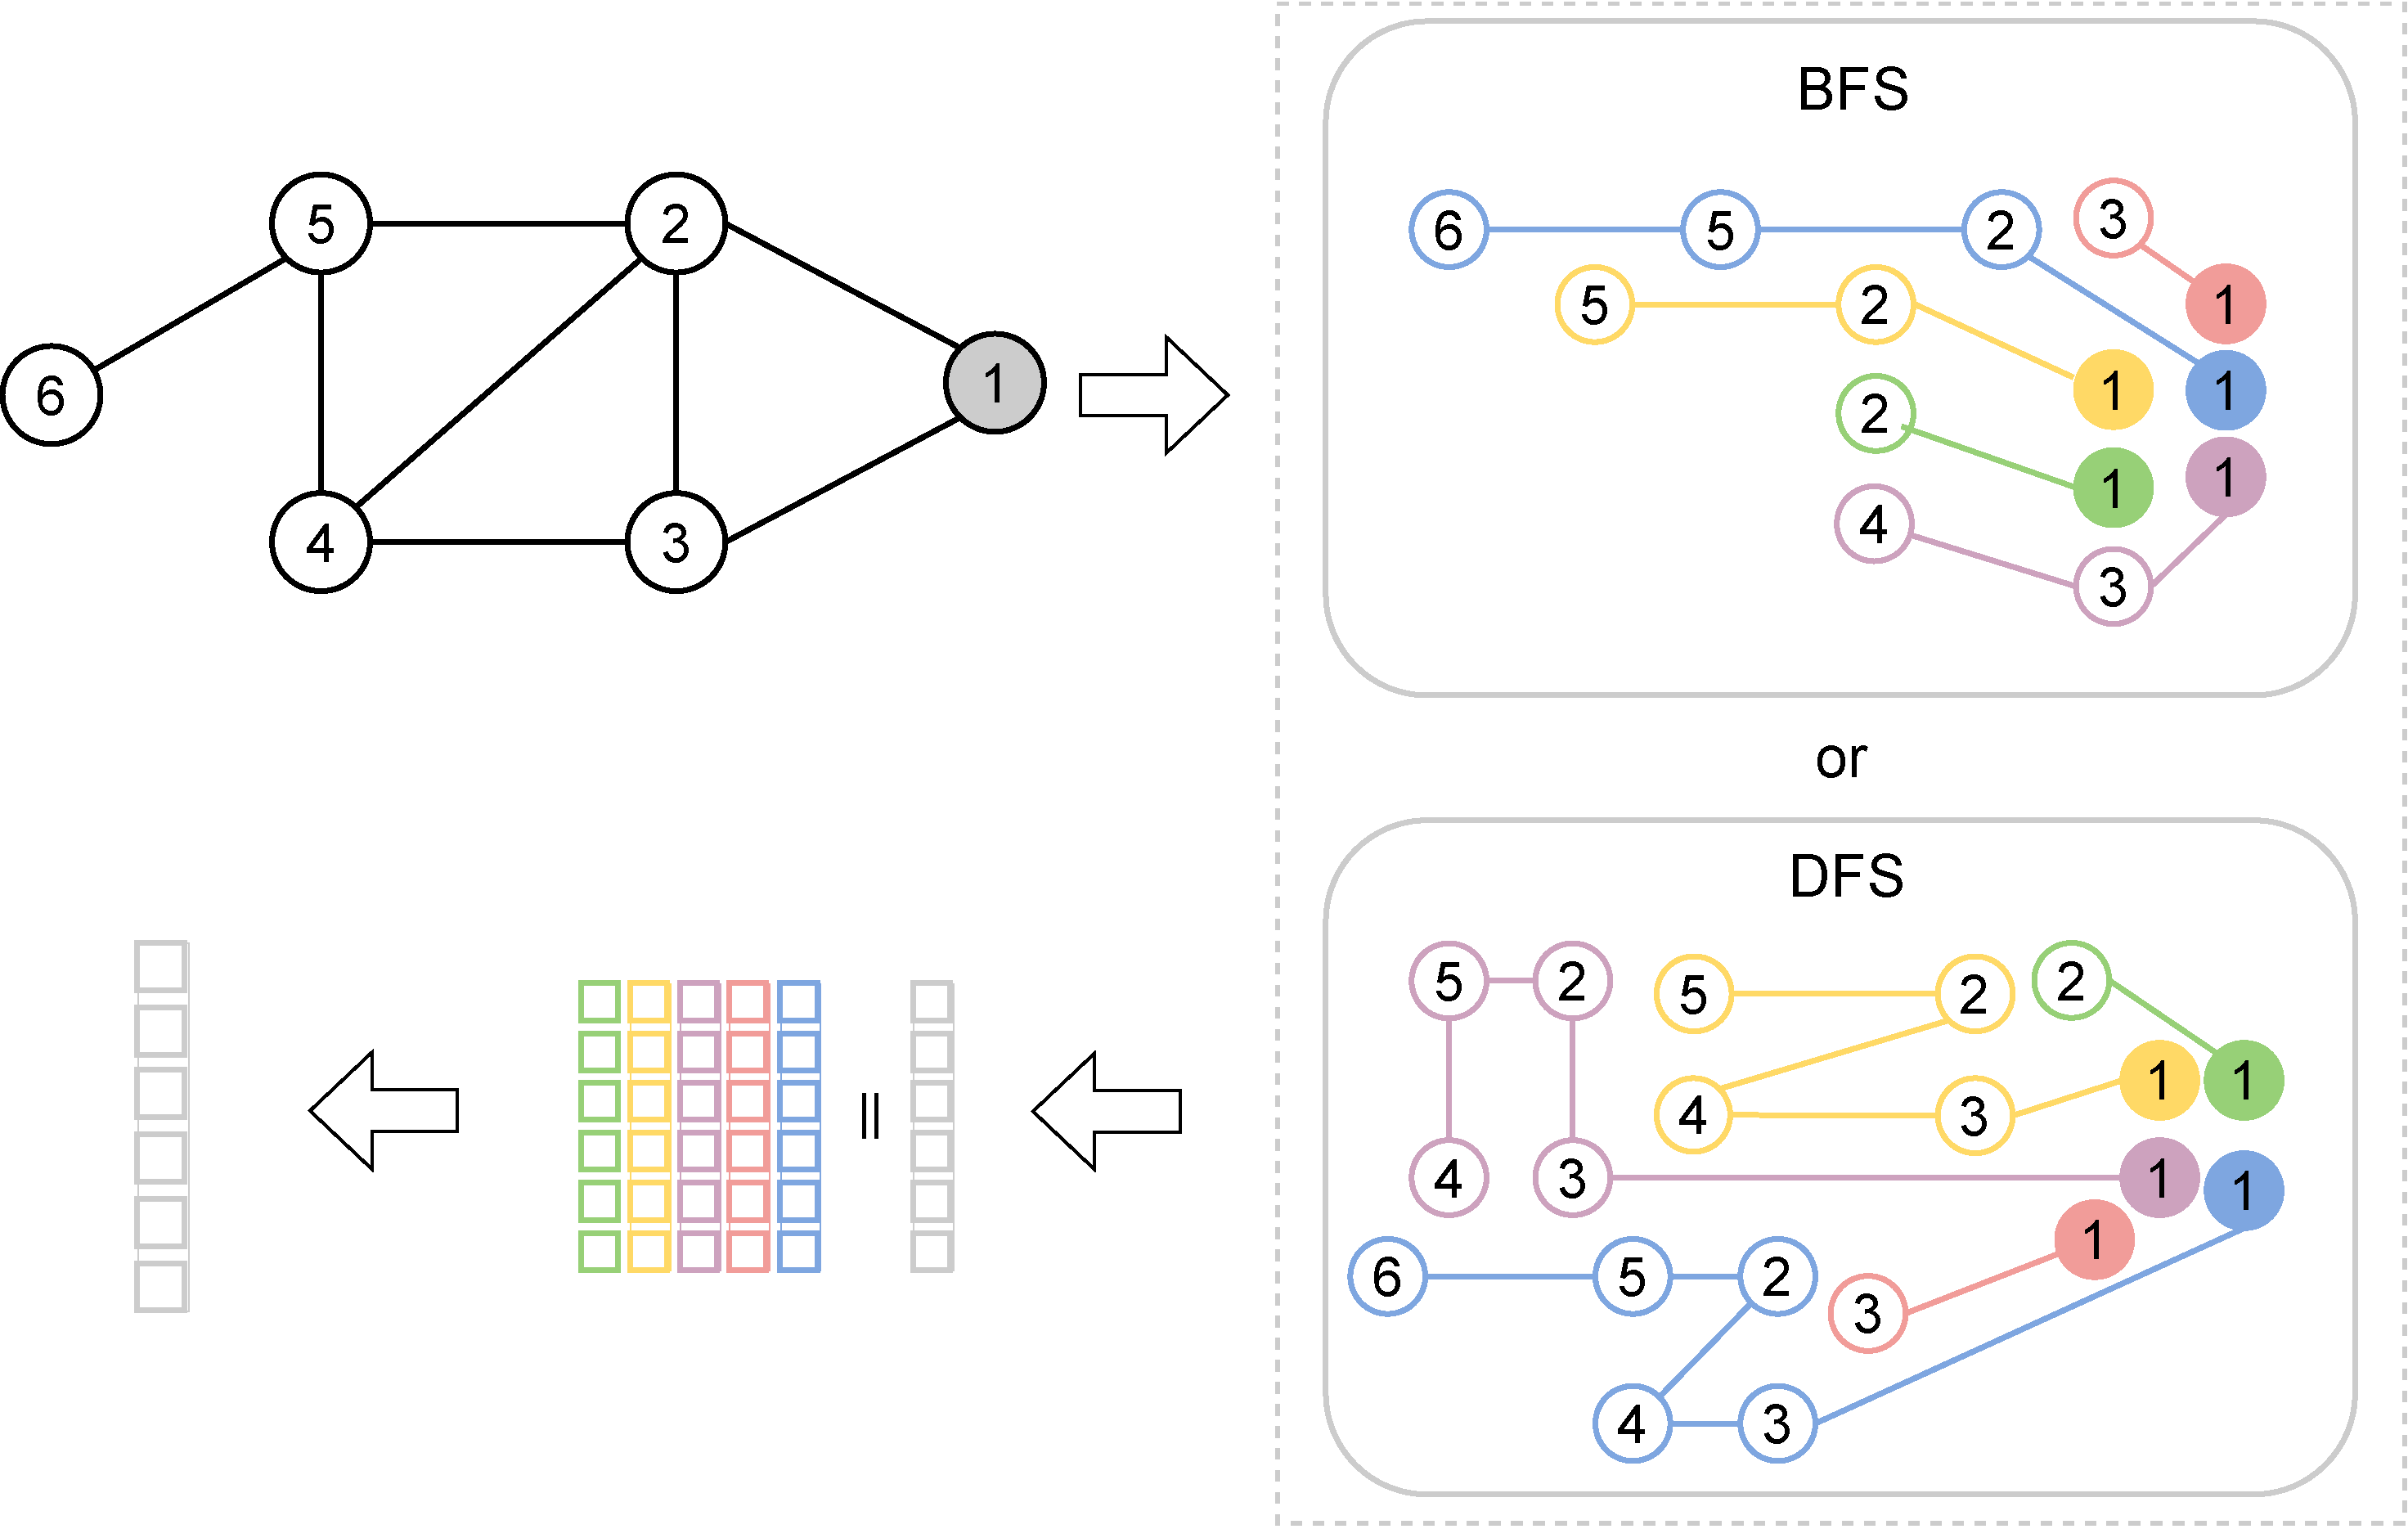
\includegraphics[clip,width=\columnwidth]{figures/localWL.pdf}
% \caption{Local vertex colouring of vertex 1}
% \label{fig:lvcgnn}
% \end{figure}
% \dw{(this section reads better than before. some notation suggestions: 1) how about using complement operation for back-edge? for example, the tree and back edges rooted from node $v$ can be $E^{v}$ and $\bar{E}^{v} = E \backslash E^{v}$, respectively?, 2)  $\varsigma$ seems not commonly used greek letter.)}\s{tree edge and back edge are directed, but $E$ is undirected, so the complement notion might cause confusions, maybe we need to define $E$ as directed too? WDYT?} \q{as the graph considered is undirected, it's better to keep $E$ undirected as well.}

In this section, we introduce the building blocks of a search-guided colouring scheme and demonstrate its expressive power in distinguishing non-isomorphic graphs. We also discuss how this search-guided colouring scheme can solve the biconnectivity and ego shortest-path graph problems that cannot be solved by MPNN. 

\subsection{Search-guided Vertex Colour Update}
We first describe a way to update vertex colours guided by graph searching. As described in \cref{sec:pre}, graph searching w.r.t. a search tree $T_v$ categorises edges into two sets: a tree edge set $E_{\text{tree}}^{T_v}$ and a back edge set $E_{\text{back}}^{T_v}$. 
Instead of propagating messages along all edges like MPNN, we design a scheme that propagates vertex information, i.e., vertex colours, along tree edges and back edges.  Given a search tree $T_v$, we define the vertex colouring refinement function on each vertex $u$ as follows
\begin{equation}
\label{eqn:lvc-all}
    \lambda^{l+1}(u):= \rho(\lambda^{l}(u), \{\!\!\{\lambda_v^{l+1}(u): v\in N_{\delta}(u)\}\!\!\})
\end{equation}
where $\rho(\cdot)$ is an injective function and $\lambda_v^{l+1}(u)$ is the vertex colour computed, based on the search tree $T_v$, as  
\begin{align}
\label{eqn:lvc}
\begin{split}
    &\lambda_v^{l+1}(u):=\\
    &\phi\left(\lambda^{l}(u), \psi\left(\{\!\!\{\lambda_v^{l}(w): w \in \eta(u, E_{\text{tree}}^{T_v}, E_{\text{back}}^{T_v})\}\!\!\}\right)\right)
\end{split}
\end{align}

where $\phi(\cdot)$ and $\psi(\cdot)$ are injective functions, %$\phi(\cdot)$ returns a colour from $C$.
and $l$ is the number of the current iteration. 
Let $\mathbb{P}(E)$ and $\mathbb{P}(V)$ be the power sets of $E$ and $V$, respectively. The function $\eta: V \times \mathbb{P}(E) \times \mathbb{P}(E) \rightarrow \mathbb{P}(V)$ takes a vertex $u\in V$ to be coloured, a tree edge set  $E_{\text{tree}}^{T_v}\in \mathbb{P}(E)$, and a back edge set $E_{\text{back}}^{T_v}\in \mathbb{P}(E)$ as input, and produces a vertex set in $\mathbb{P}(V)$. 


At the first iteration, $\lambda^0_v(w)$ and $\lambda^0(w)$ are the initial colours of $w$. There are two steps in the colouring scheme. The first step is \emph{search-guided colour propagation}
(\cref{eqn:lvc}), where vertex colours are propagated along the search paths of each $T_v$ based on $\eta(u, E_{\text{tree}}^{T_v}, E_{\text{back}}^{T_v})$. After this step, a vertex $u$ obtains a colour $\lambda^{l+1}_v(u)$ w.r.t. each root vertex $v\in N_{\delta}(u)$. We obtain in total $|N_{\delta}(u)|$ colours for $u$. The second step is \emph{neighbourhood aggregation} (\cref{eqn:lvc-all}), where the $|N_{\delta}(u)|$ colours obtained from the first step are aggregated and used to compute a new colour $\lambda^{l+1}(u)$ for $u$. These two steps are repeated with the new vertex colours.
 
When $N_\delta(v) \neq V$, we call this vertex colouring scheme \emph{$\delta$-local vertex colouring} (LVC-$\delta$).
LVC-$\delta$ is applied to colour vertices in $G$ iteratively until vertex colours are stabilised.
We omit superscript and use $\lambda$ to refer to a stable colouring.



% We first describe two ways to update vertex colour in graph searching.  A graph searching method visits each vertex one at a time; at each visit, it finds a \q{search (tree?)} edge and perhaps one or more back edges. At the end of searching, the \q{search (tree?)} edges form a search tree rooted at the starting point $v$. The first way to update vertex colour is what we call a \textit{forward-update} which colours vertices along searching when visiting each vertex.
% \begin{definition}
%     A \textbf{forward-update} assigns colours to vertices at each search visit, using the currently available search paths and back edges.
% \end{definition}
% Forward-update aligns well with graph algorithms that are analogous to dynamic programming, such as Dijkstra, Floyd-Warshall, and Bellman-Ford. \dw{(why?)}

% The second way to update vertex colour is what we call a \textit{backward-update} which updates vertex colours at the end of searching.
% Back-update allows vertex colour to be updated using information from the entire search. which aligns with algorithms that backtracks the search tree like Tarjan's algorithm. \q{(add citations for the algorithms mentioned in this paragraph)}
% \begin{definition}
%     A \textbf{backward-update} assigns colours to vertices the end of search, using the entire search tree and back edges.
% \end{definition}

% \q{(Maybe better to change "forward-update/backward-update" to formard-colouring/backward-colouring schemes)}

\paragraph{Search order permutation.}
Graph searching may encounter cases where a search algorithm needs to decide a priority between two or more unvisited vertices (a tie). In such cases, the search algorithm can visit any vertex in the tie. This yields different vertex visiting orders, we call this permutation in vertex visiting order \textit{search order permutation}. 
For example, in \cref{subfig:edge_type_b}, the BFS rooted at vertex $v_0$ faces a tie, where it can visit either $v_1$ or $v_2$ first since both $v_1$ and $v_2$ are adjacent to $v_0$. \cref{subfig:edge_type_b} shows the search trajectory when visiting $v_1$ first; however, if the BFS visits $v_2$ first, then tree edges and back edges will be different. 

\paragraph{Design considerations.}
A key function that controls the colouring in \autoref{eqn:lvc} is $\eta$. For instance, we can make LVC-$\delta$ identical to 1-WL, if we define $\eta(u, E_{\text{tree}}^{T_v}, E_{\text{back}}^{T_v}) = \{w:(u,w) \in E_{\text{tree}}^{T_v}\vee (w,u) \in E_{\text{tree}}^{T_v}\vee (u,w) \in E_{\text{back}}^{T_v} \vee (w,u) \in E_{\text{back}}^{T_v}\}$. We name it \emph{1-WL-equivalent LVC}. In this definition, $\eta$ effectively yields all neighbouring vertices of $u$, making it equivalent to 1-WL. 

Since the design of $\eta$ is crucial, we hereby introduce two key points that should be considered when designing $\eta$. 
\begin{itemize}
    \item $\eta$ should be invariant to search order permutation, i.e. a change of vertex visiting order should not alter the output of $\eta$. If $\eta$ is not invariant to search order permutation, the colouring scheme will not be permutation invariant. The 1-WL equivalent LVC example in the previous paragraph is invariant to search order permutation. 
    \item $\eta$ should inherit properties of a search algorithm that are informative about identifying graph structure. Graph searches like BFS and DFS are widely used in graph algorithms to capture structural properties such as cycles and biconnectivity. $\eta$ should be designed to incorporate such structural information in vertex colours.
\end{itemize}

% Apart from search order permutation, the choice of root $v$ is another factor of variance, as search trees rooted at different vertices can be vastly different. Unless we have a pre-determined canonical ordering of vertices (which is possible for some domain-specific applications), to colour a vertex $u$, we need to perform searching rooted at all vertices $v \in N_{\delta}(u)$.
% \begin{equation}
% \label{eqn:lvc-all}
%         \lambda^{l+1}(u):= \rho(\lambda^{l}(u), \{\!\!\{\lambda_v^{l+1}(u): v\in N_{\delta}(u)\}\!\!\})
% \end{equation}
% where $\rho(\cdot)$ is an injective function. When the search is limited to $N_\delta(v)$, we call it $\delta$-local vertex coloring (LVC\textsuperscript{$\delta$}).
% %Same to other vertex colour refinement algorithms, we may apply



\begin{figure}[t!]
\centering
\begin{subfigure}{.44\columnwidth}
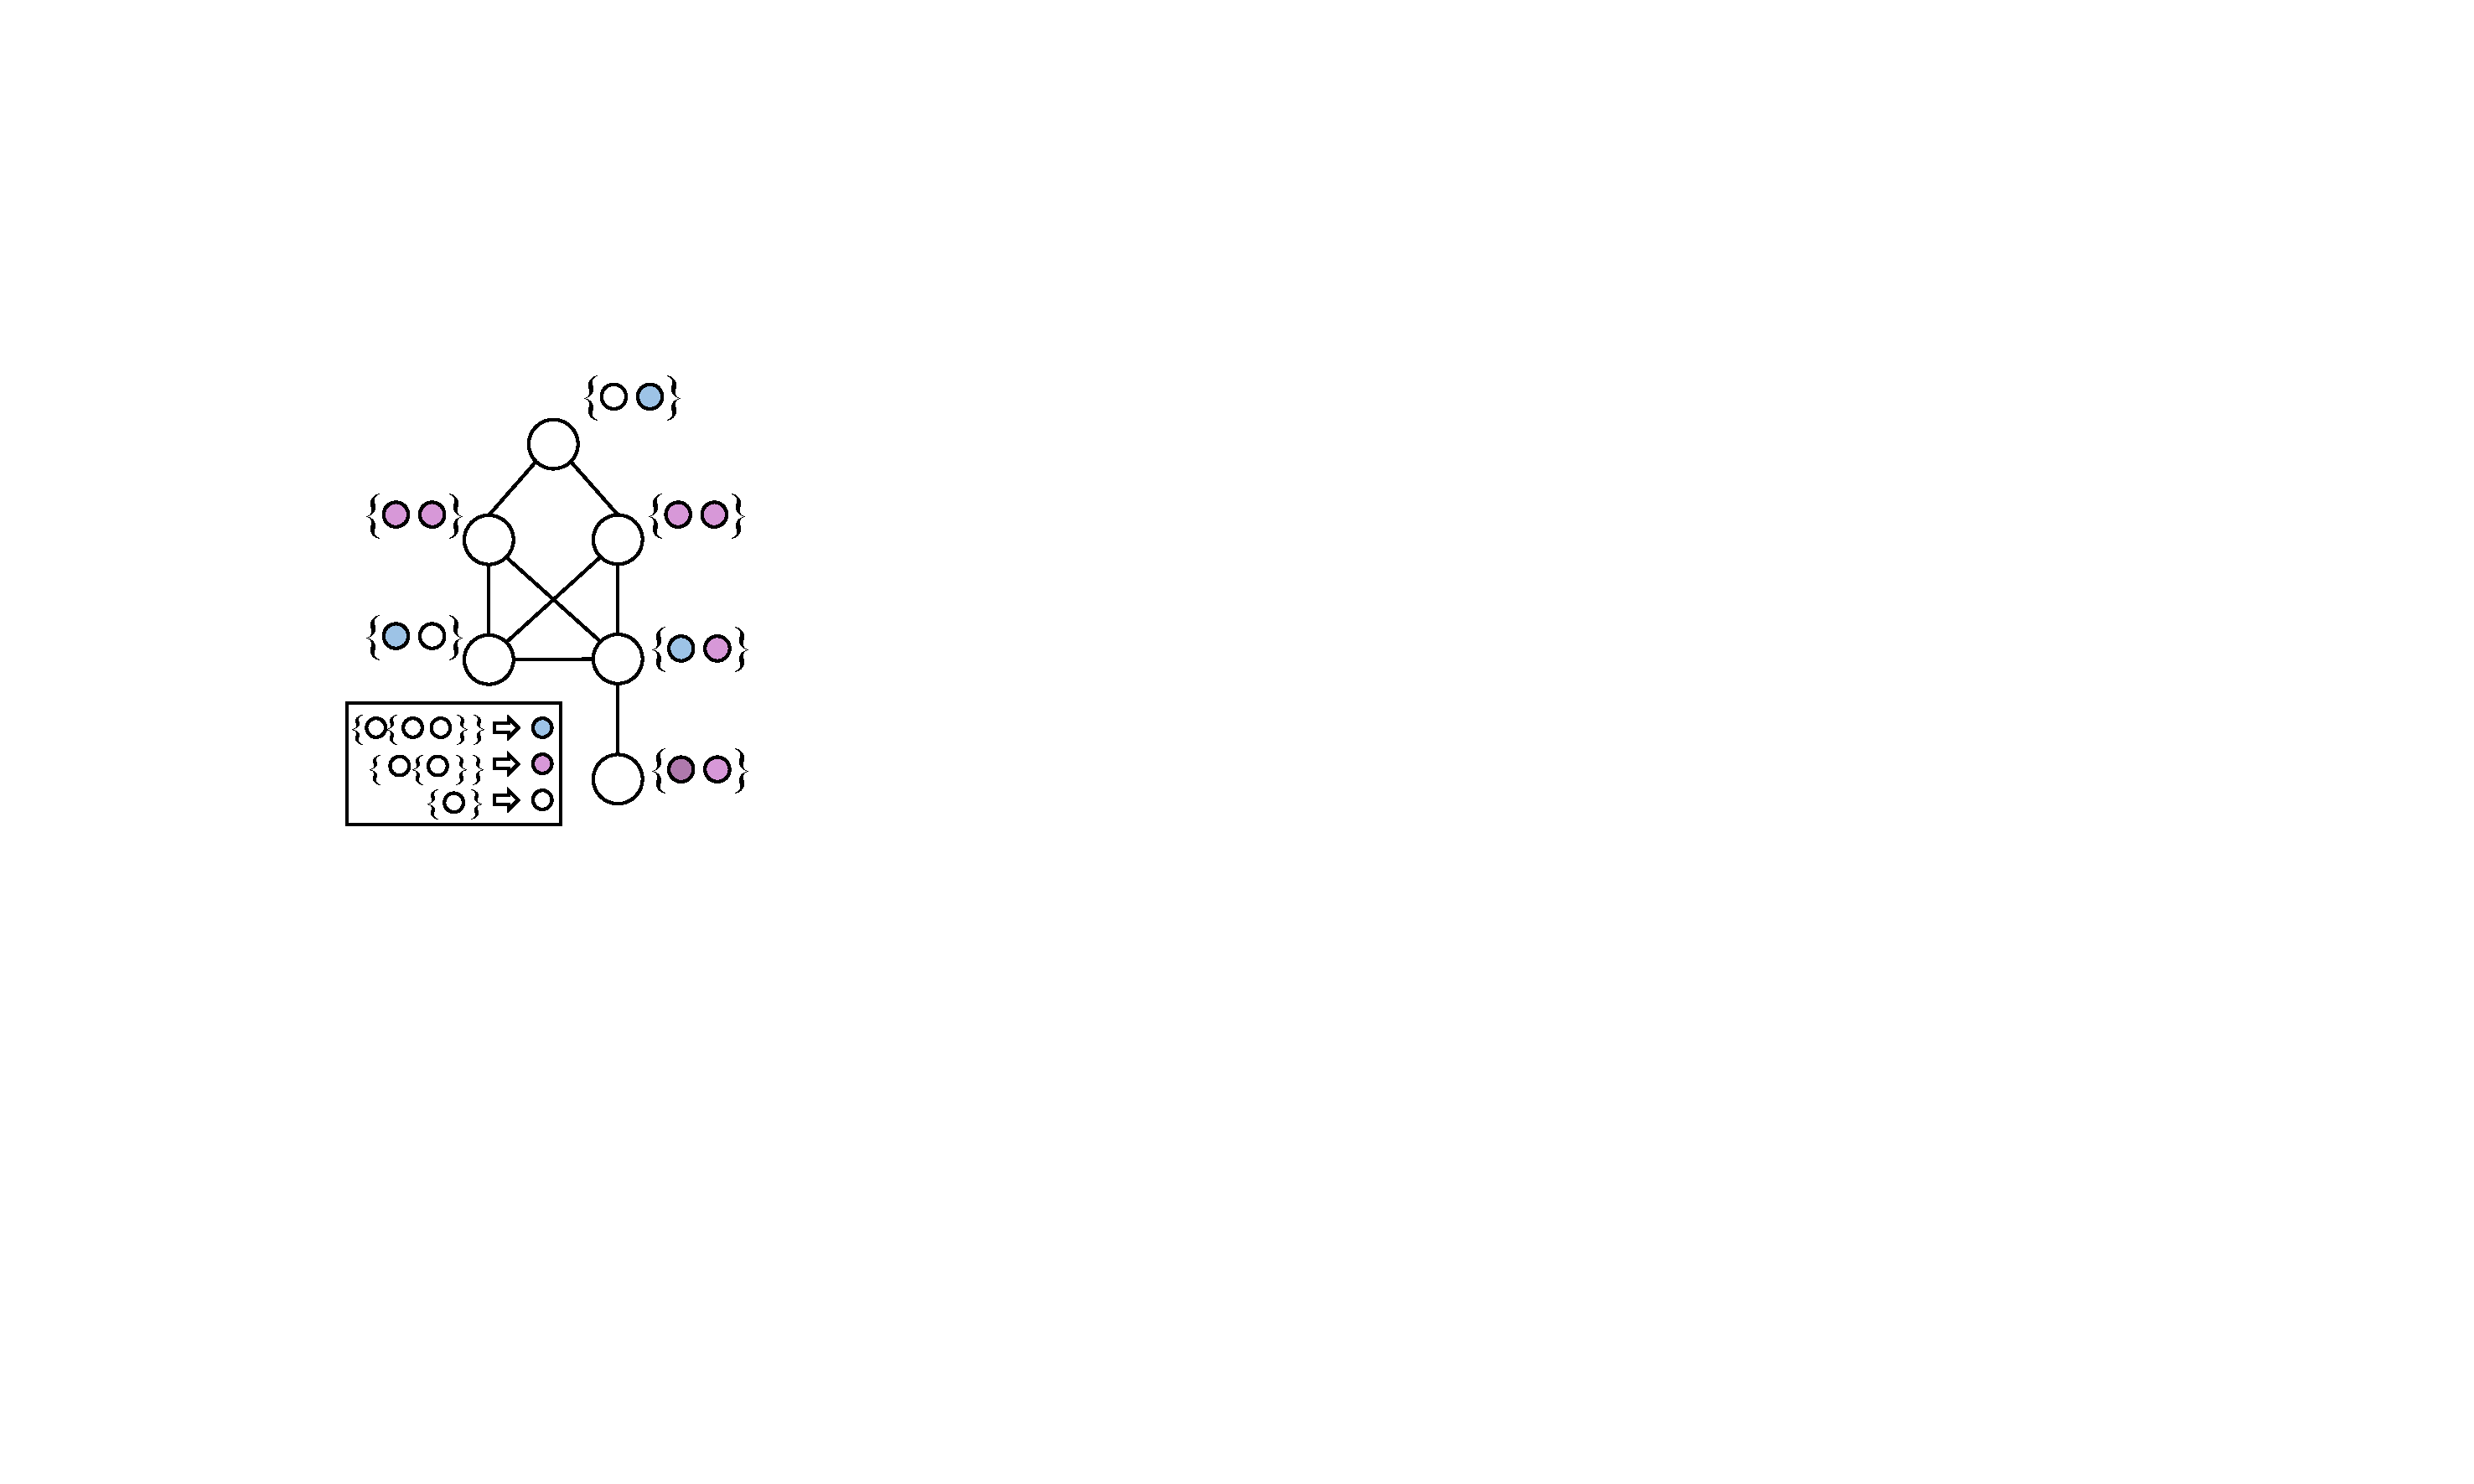
\includegraphics[clip,width=\textwidth]{figures/bfc_1_new.pdf}
\subcaption{}
\label{subfig:bfc1}
\end{subfigure}%
\hfill
\begin{subfigure}{.25\columnwidth}
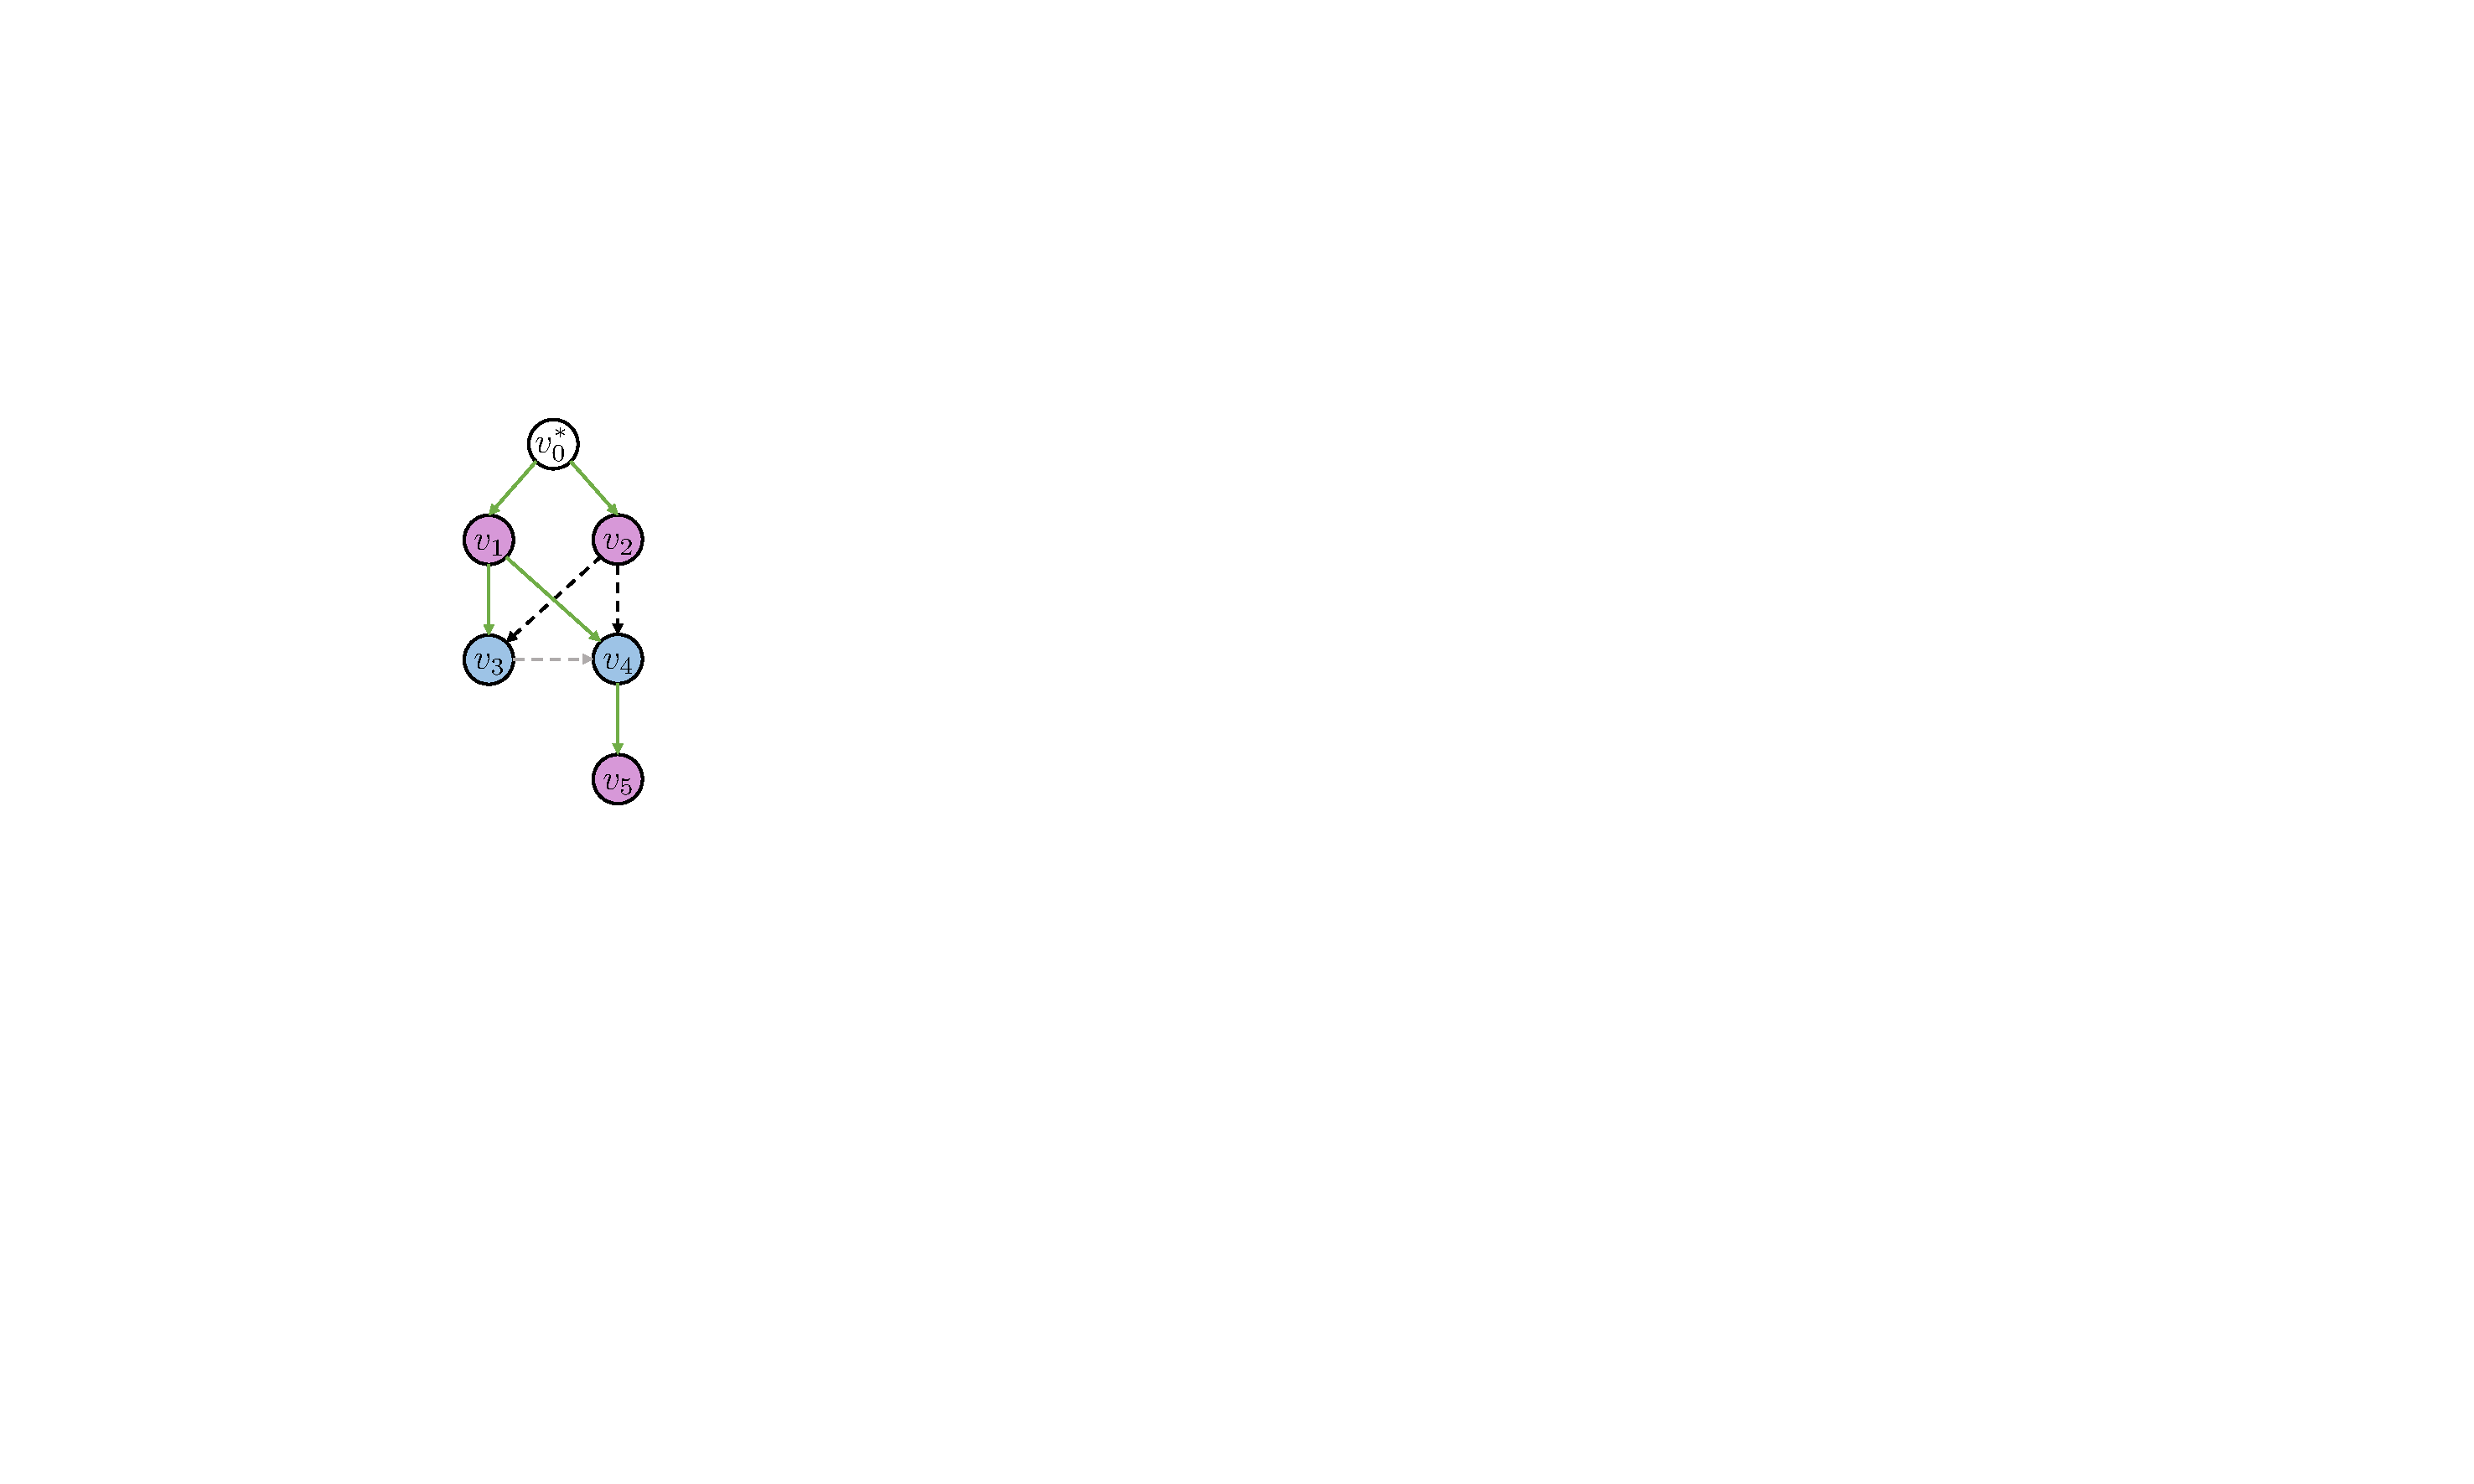
\includegraphics[clip,width=\textwidth]{figures/bfc_2_new.pdf}
\subcaption{}
\label{subfig:bfc2}
\end{subfigure}
\hfill
\begin{subfigure}{.25\columnwidth}
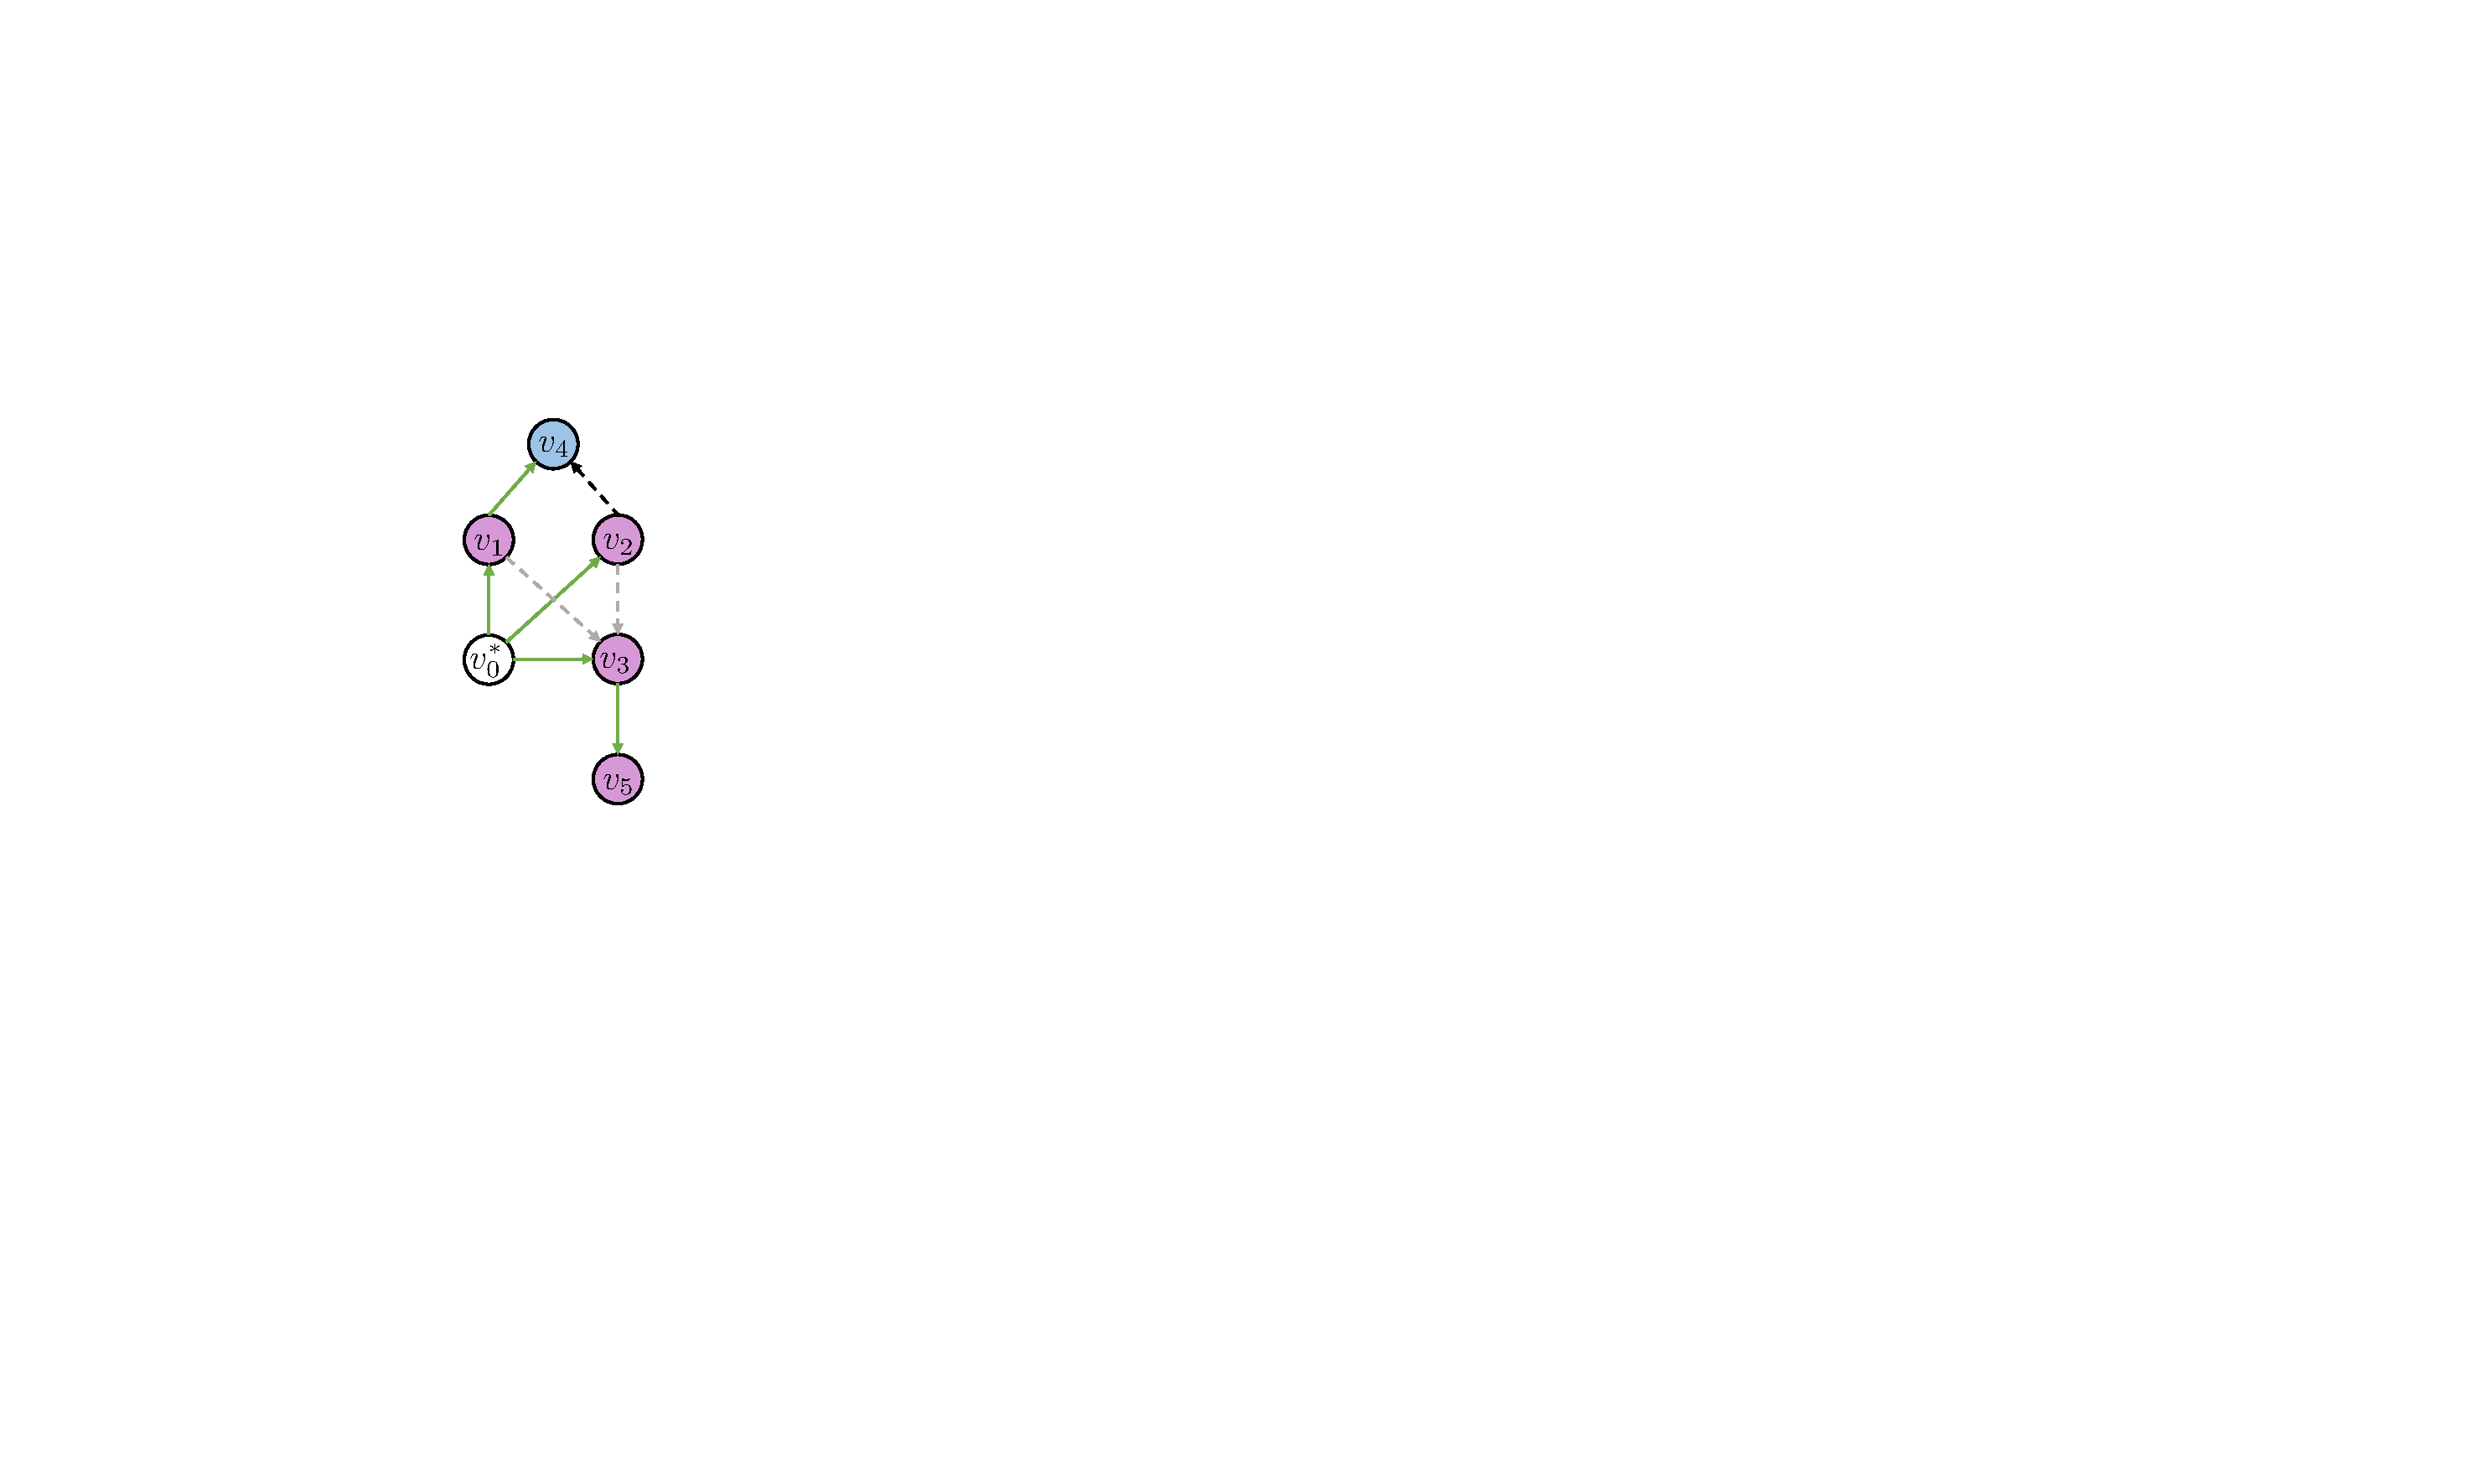
\includegraphics[clip,width=\textwidth]{figures/bfc_3_new.pdf}
\subcaption{}
\label{subfig:bfc3}
\end{subfigure}
\caption{
A graph and its vertex colours after the first BFC iteration. \ref{subfig:bfc1} shows the uncoloured graph, where the vertex colours obtained from \ref{subfig:bfc2} and  \ref{subfig:bfc3} are shown next to each vertex. 
\ref{subfig:bfc2} and \ref{subfig:bfc3} show BFC with two different roots (marked with *), respectively, where each vertex is assigned a new colour by BFC. The colour map is shown in the bottom left corner. The subscripted labels $v_0$, \dots, $v_5$ denote the visit sequence of each vertex, e.g. $v_1$ is visited after $v_0$.
For brevity, we show BFC with only two roots.} 
\label{fig:bfc}
\end{figure}

\subsection{BFS-guided Colouring}
BFS is perhaps the most widely used graph search algorithm and its applications include finding shortest paths, minimum spanning tree, cycle detection, and bipartite graph test. We design $\eta$ for BFS, denoted as $\eta_{\text{bfc}}$, as 
\begin{align}
%\begin{split}
\label{eqn:sigma_bf}
    &\eta_{\text{bfc}}(u, E_{\text{tree}}^{T_v}, E_{\text{back}}^{T_v}) =& \\
     &\left\{o: (o,u) \in E_{\text{tree}}^{T_v} \vee 
    \left((o, u) \in E_{\text{back}}^{T_v} \wedge
    d(v,o) \neq d(v,u)\right)
    \right\}& \notag
%\end{split}
\end{align}
The part $\{o: (o,u) \in E_{\text{tree}}^{T_v}\}$ preserves vertices that lead to vertex $u$ via tree edges. $\{o: (o, u) \in E_{\text{back}}^{T_v}\}$ preserves vertices that lead to vertex $u$ via back edges. The condition $d(v,o) \neq d(v,u)$ ensures only back edges connecting vertices at different levels are included.
The vertex colouring scheme using $\eta_{\text{bfc}}$ is called \textit{breadth-first colouring} (BFC).

\cref{fig:bfc} shows BFC rooted at two different vertices, where the grey dashed lines indicate back edges that are excluded by BFC. In \cref{subfig:bfc2}, when $u = v_4$, $\eta_{\text{bfc}}$ returns $v_1$ and $v_2$, but excludes $v_3$ because it is at the same level as $v_4$. 
% Sean revised here

An important property of BFS is that tree edges form the shortest paths between a root to other vertices, e.g., in \cref{subfig:bfc2} $(v_0,v_1)$ and $(v_1,v_4)$ form the shortest path $(v_0,v_1,v_4)$ between $v_0$ and $v_4$. 
There are two categories of back edges in a BFS tree: the ones connecting vertices across two adjacent levels and the ones connecting vertices at the same level~\citep{Cormen_algointro}. The first category of back edges forms alternative shortest paths, e.g., $(v_0,v_2)$ and $(v_2,v_4)$ form another shortest path $(v_0,v_2,v_4)$ between $v_0$ and $v_4$. The second category of back edges does not participate in any shortest path. %: if a path contains the second category of back edge, its distance will increase by one compared to the shortest paths formed by only tree edges.
$\eta_{\text{bfc}}$ only preserves the first category of back edges and excludes the second category by the condition $d(v,o) \neq d(v,u)$. 
All shortest paths from a root to a vertex, e.g., $(v_0,v_1, v_4)$ and $(v_0,v_2,v_4)$, form an induced shortest path graph (SPG)~\citep{Wang2021-shortestpathgraph}, which is permutation invariant. For example, if we swap the search order between $v_1$ and $v_2$ in \cref{subfig:bfc2}, $(v_1,v_4)$ becomes a back edge and $(v_2,v_4)$ becomes a tree edge, but $\eta_{\text{bfc}}$ returns the same vertex set. Hence, BFC defined by Equations \ref{eqn:lvc-all}, \ref{eqn:lvc}, and \ref{eqn:sigma_bf} is also permutation invariant. 

BFC is referred as BFC-$\delta$ if the search range is limited to a $\delta$-hop neighbourhood for each root vertex. 


% The \q{out-of-box BFS tree edges (?)} are neither invariant or equivariant: \q{there could be many shortest paths between two vertices, the one in a BFS search tree is one of many legit choices. (I probably understand your intention here but it would be hard for others to follow - why suddenly it jumps from BFS 
% (as a general search algorithm) to shortest paths (a specific problem)} However, we can form all shortest paths between two vertices by including back edges (a back edge indicates a cycle, and there can be more than one shortest path between vertices on a cycle). 

% \q{(general comments: it would be better to describe the BFS colouring only based on the traversal and tree/back edges, while leaving the connections to shortest paths as the consequence of this colouring scheme.)}

% Intuitively, we design the forward-update in such way that the colour of root $v$ propagates along the search paths, while a vertex $u$ is visited on the path, the propagated colour combines with the existing colour of $u$, and gets assigned to $u$ before it propagates further down the path.
% Formally, let $(G, \lambda)$ be a vertex-coloured graph with an initial colouring $\lambda(v)$ for $v\in V$, $\lambda_v(u)$ denote the colour of vertex $u$ w.r.t. a root vertex $v$. \q{(some consistency/clarity of notations w.r.t. Equation 1 needs to be checked)}
% When visiting $u$, the edge leads to $u$ is added to the tree edge set $E_{tree}$ and the back edges start from $u$ are added the the back edge set $E_{\text{back}}$.
% In BFS, a back edge can only exist between two vertices on the same level or adjacent levels. It is easy to see the other shortest-paths not in the search tree must contain a back edge between adjacent levels. A simple proof is if a path contains a back edge between two vertices on the same level, its distance will increase by 1 comparing to the shortest path formed by only tree edges. We include \q{between-level back edge} in the forward-update. Adding the same-label back edges would break invariance, so we leave them out.

% Vertex colour in updated in forward-update according to
% \begin{equation}
% \label{eqn:bfs_lvc_forward}
%     \lambda_v(u):= \phi\Bigl(\lambda(u), \psi\bigl(\{\!\!\{\lambda_v(w): w \in \mathbb{B}_u\}\!\!\}\bigr)\Bigr) \quad \text{(BFS forward-update)}
% \end{equation}
% where $\phi(\cdot)$ and $\psi(\cdot)$ are injective functions that returns a colour from $C$, initially, $\lambda_v(v):=\lambda(v)$. \q{$\mathbb{B}_u$ is the set of vertices that proceeds $u$ in tree edges or succeeds $u$ in back edges.(discuss)}
% \begin{equation*}
%     \mathbb{B}_{u}:= \{o: (o,u) \in E_{\text{tree}}\text{ or } 
%     (u, o) \in E_{\text{back}} \text{ and } 
%     d_{vo} \neq d_{vu}
%     \}
% \end{equation*}

% We call \cref{eqn:bfs_lvc_forward} the \textit{BFS forward-update}. 
% We name the BFS-guided LVC using \cref{eqn:bfs_lvc_forward} as LVC-BFS.
% We treat \textit{BFS backward-update} as a no-op and ignore it in this LVC-BFS.


% Given a root vertex $v\in V$, the \emph{Local Vertex Colouring} (LVC) algorithm starts at the root vertex $v$ and traverses to vertices in its neighbourhood $N_{\delta}(v)$ recursively in increasing order of their distances to the root vertex. For each vertex being visited, a colour is assigned based on the multiset of colours of its adjacent neighbours that have been visited and relative position between the vertex and $v$.


% Intuitively, colour of $v$ is carried to $u$ along the path $\mathcal{P}^{\mathcal{T}}_{vu}$ together with colour of other vertices also on $\mathcal{P}^{\mathcal{T}}_{vu}$.
% Yet, different search approaches might yield different paths that further affect expressity of the model. We hereby define a type of search that guarantees a hierarchical expressivy power with respect to $\delta$.

\paragraph{Distinguishing shortest-path graphs.} 
\citet{Velickovic_neuralexecutoin} show that MPNN can imitate classical graph algorithms to learn shortest paths (Bellman-Ford algorithm) and minimum spanning trees (Prim’s algorithm). \citet{xu20_gnnreasoning} further show that MPNN is theoretically suitable for learning tasks that are solvable using dynamic programming. Since the base form of BFC (i.e. BFC-1) aligns with MPNN (will be discussed later), BFC also inherits these properties. However, we are more interested in tasks which BFC can do but MPNN cannot. We show that one of such tasks is to distinguish ego shortest-path graphs. 

\begin{definition}
For two vertices $v, u\in V_G$, a \emph{shortest-path graph} $SPG(v,u)$ is a subgraph of $G$, where $SPG(v,u)$ contains all and only vertices and edges occurring in the shortest paths between $u$ and $v$.
\end{definition}

\begin{restatable}[]{lemma}{bfcspg}
\label{lemma:bfc2spg}
Let $(u,v)$ and $(u',v')$ be two pairs of vertices. Then $SPG(u,v)\simeq SPG(u',v')$ if and only if one of the following conditions hold under BFC: (1) $\lambda_v(u)= \lambda_{v'}(u')$ and $\lambda_u(v)= \lambda_{u'}(v')$; (2) $\lambda_v(u)= \lambda_{u'}(v')$ and $\lambda_u(v)= \lambda_{v'}(u')$.
\end{restatable}

\begin{definition}
Given a vertex $v\in V_G$ and a fixed $\delta \geq 1$, an \emph{ego shortest-path graph} (ESPG) $S_v = (V_{S_v}, E_{S_v})$ is a subgraph of $G$, where $V_{S_v} = N_{\delta}(v)$ and $E_S$ is the set of all edges that form all shortest paths between $v$ and $u\in N_{\delta}(v)$.
\end{definition}

%\begin{restatable}[]{lemma}{lvcbfsesgp}
%\label{lemma:lvcbfs_esgp}
%For any two vertices $v \in V_G$ and $u \in V_H$, and their ESPG $S_v$ and $S_u$, we have $S_v\simeq S_u$ if and only if $\lambda_G(v) = \lambda_H(u)$ after running BFC.
%\end{restatable}

%\q{(I think there is no need to consider $v$ and $u$ are in different graphs $G$ and $H$. This makes the notations unnecessarily complicated, for example, you may have the following: )}and 

\begin{figure}[ht]
\centering
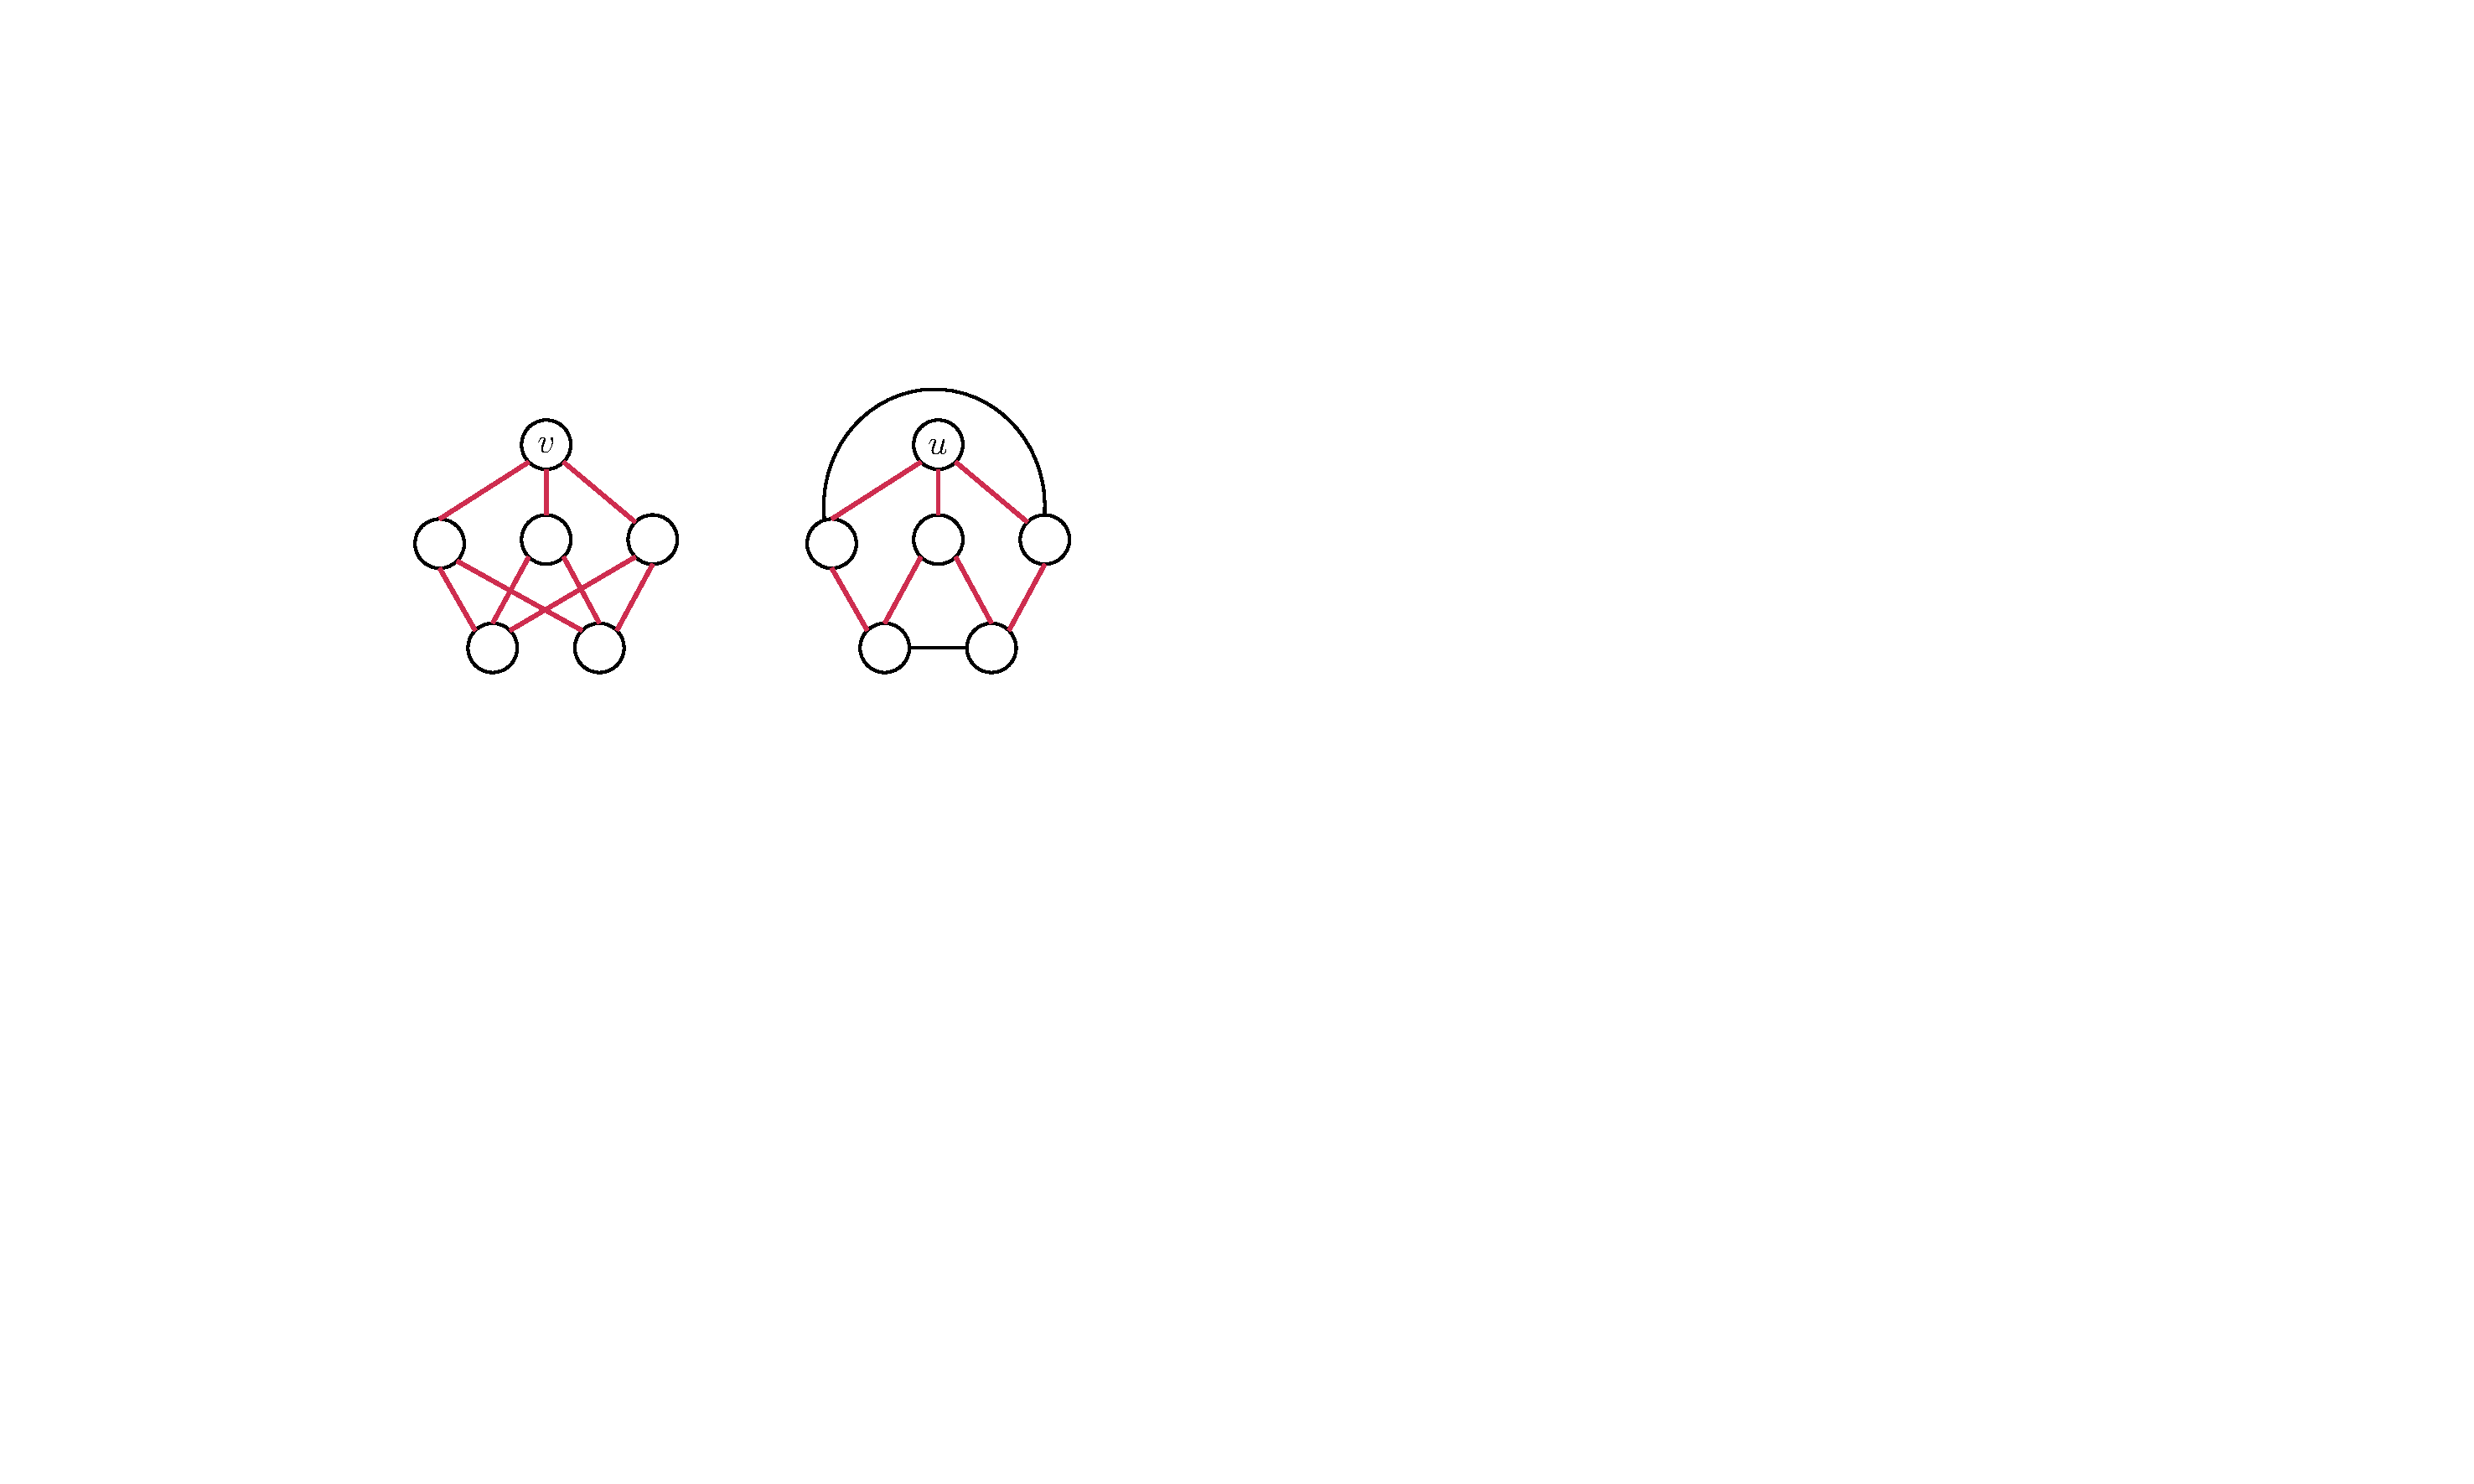
\includegraphics[clip,width=0.65\columnwidth]{figures/lemma2_a_new.pdf}
\caption{A pair of non-isomorphic three-regular graphs. Pink edges form ESPGs ($\delta = 2$) for vertices $v$ and $u$.} 
\label{fig:esgp_examples}
\end{figure}

\begin{restatable}[]{lemma}{lvcbfsesgp}
\label{lemma:lvcbfs_esgp}
Let $v,u \in V$ be any two vertices and $\lambda(v)$ and $\lambda(u)$ be the corresponding stable colours of $v$ and $u$ by running BFC.  We have $S_v\simeq S_u$ if and only if $\lambda(v) = \lambda(u)$, where $S_v$ and $S_u$ are the ESPGs of $v$ and $u$, respectively. 

%\q{(notes from qing: stable colours only happen when there is no any further change)}
\end{restatable}

\begin{restatable}[]{lemma}{mpnnesgp}
\label{lemma:mpnn_esgp}
MPNN cannot distinguish one or more pairs of graphs that have non-isomorphic ESPGs.
 %\sout{for any two vertices $v \in V_G$ and $u \in V_H$, and their ESPG $S_v$ and $S_u$. Let $h_v$ and $h_u$ be the vertex representations of $v$ and $u$ by MPNN, when $h_v = h_u$, $S_v\simeq S_u$ may not hold. Similarly, when the $S_v\simeq S_u$, $h_v = h_u$ may not hold.}
\end{restatable}
\cref{fig:esgp_examples} shows a pair of graphs with non-isomorphic ESPGs that BFC is able to distinguish but MPNN cannot.

%\q{(For a lemma like the above, you only need to show a counterexample to prove it. The orignal statement is also too lengthy)}

%\begin{restatable}[]{corollary}{lvcbfspathlength}
%\label{corollary:lvc_bfs_path_distance}
%BFC implicitly encodes search path length, i.e. For any two vertices $v \in V_G$ and $u \in V_H$, $\lambda_G(v) = \lambda_H(u)$ only if for each $v'\in N_{\delta}(v)$ there is a $u'\in N_{\delta}(u)$ such that $|P_{v'v}| = |P_{u'v}|$, and vice versa.
%\end{restatable}

%\q{(same for the above corollary, it can be simplified as)}


% \begin{algorithm}[th]
% \caption{$\text{Modified BFS (mBFS)}(G, v, w, \delta, \lambda, \lambda_v(w))$}
% \label{alg:search_and_colour}
% \begin{algorithmic}[1]
% \STATE {\bfseries Input:} Graph $G$, root vertex $v$, current vertex $w$, search radius $\delta$, vertex colour $\lambda$, vertex colour $\lambda_v$, 
% \STATE {\bfseries Output:} Updated vertex colour $\lambda_v$
% \STATE $u \gets \text{next}(G, w)$
% \IF{$d_{vu}\leq \delta$}
% \STATE $\lambda_v(u) \gets \texttt{hash}(\lambda(u), \lambda_v(w))$
% \STATE $\text{search\_and\_colour}(G, v, u, \delta, \lambda, \lambda_v)$
% \ENDIF
% \end{algorithmic}
% \end{algorithm}

\subsection{DFS-guided Colouring}
%Similar to BFS, 
DFS is also a fundamental graph search method for graph problems, including detecting cycles, topological sorting, and biconnectivity.
Unlike BFS whose search range grows incrementally by hop, DFS explores vertices as far as possible along each branch before backtracking. 
Before introducing a DFS-guided vertex colouring, recalling that we must have $v_j\prec v_i$ (or $i>j$) for any DFS back edge $(v_i, v_j)$, we introduce two concepts used in defining $\eta$ for DFS. 

%\begin{definition}[Back edge crossover]
%We define a relation between back edges, $\nmid$, referred to as ``crossover",  on $E_{\text{back}}^{T_v}$, assume $\vec{e}_1 = (v_{i_1}, v_{j_1})$, $\vec{e}_2=(v_{i_2}, v_{j_2})$, 
%\begin{equation}
%    \vec{e}_1 \nmid \vec{e}_2, \forall \vec{e}_1,\vec{e}_2\in E_{\text{back}}^{T_v}
%\end{equation}
%if one of the two conditions is satisfied:
%\begin{enumerate}
%    \item  $j_2 \leq j_1 < i_2 < i_1$
%    \item  $j_1 < j_2 < i_1 \leq i_2$
%\end{enumerate}
%\end{definition}

\begin{definition}[Back edge crossover]
Let $T_v$ be a search tree rooted at vertex $v\in V$ and $E_{\text{back}}^{T_v}$ be the set of back edges of $T_v$. A relation \emph{crossover} $\nmid$ on $E_{\text{back}}^{T_v}$ is defined as $\vec{e}_1 \nmid \vec{e}_2$, where $\vec{e}_1 = (v_{i_1}, v_{j_1})$ and $\vec{e}_2=(v_{i_2}, v_{j_2})$,
if one of the following four conditions is satisfied:
\begin{enumerate}
    \item[(1)]  $j_2 < j_1 < i_2 < i_1$
    \item[(2)]  $j_1 < j_2 < i_1 < i_2$
    \item[(3)]  $j_1 = j_2\text{, }i_1 \neq i_2$
    \item[(4)]  $i_1 = i_2\text{, }j_1 \neq j_2$
\end{enumerate}
\end{definition}
It is easy to see that $\nmid$ is symmetric. That is, $\vec{e}_2 \nmid \vec{e}_1$  if and only if $\vec{e}_1 \nmid \vec{e}_2$. For instance, in \cref{subfig:dfc2} we have $(v_2,v_0)\nmid (v_3,v_1)$. In \cref{subfig:edge_type_c}, we have $(v_3,v_1)\nmid (v_5,v_2)$ and $(v_5,v_0)\nmid (v_5,v_2)$. 

%\begin{definition}[Back edge cover]
%We define a relation between a vertex and a back edge, $\dashv$, referred to as ``covered by", on $v$ and $\vec{e} \in E_{\text{back}}^{T_v}$, assume a back edge $\vec{e} = (v_{i}, v_{j})$, and a vertex $v_{k}$, 
%\begin{equation}
 %   v_k \dashv \vec{e}, \forall \vec{e}\in E_{\text{back}}^{T_v}, v \in V
%\end{equation}
%if and only if  $v_k \in \mathcal{P}^{T_v}_{v_jv_i}$, where $\mathcal{P}^{T_v}_{v_jv_i}$ is a path from $v_j$ to $v_i$, formed by tree edges in the search tree $T_v$.
%\end{definition}


\begin{definition}[Back edge cover]
Let $v\in V$ be a vertex, $T_v$ be a search tree rooted at vertex $v$, $\vec{e} \in E_{\text{back}}^{T_v}$ be a back edge of $T_v$, and $\vec{e} = (v_{i}, v_{j})$. We say that $v$ is \emph{covered by} $\vec{e}$, denoted as $v \dashv \vec{e}$,
if and only if  $v \in \mathcal{P}^{T_v}_{v_jv_i}$, where $\mathcal{P}^{T_v}_{v_jv_i}$ is a path from $v_j$ to $v_i$, formed by tree edges of $T_v$.
\end{definition}
In \cref{subfig:edge_type_c}, we have $v_2 \dashv(v_3,v_1)$. In \cref{subfig:dfc3}, we have $v_1 \dashv (v_2, v_0)$. 


\begin{figure}[t!]
\centering
\begin{subfigure}{.42\columnwidth}
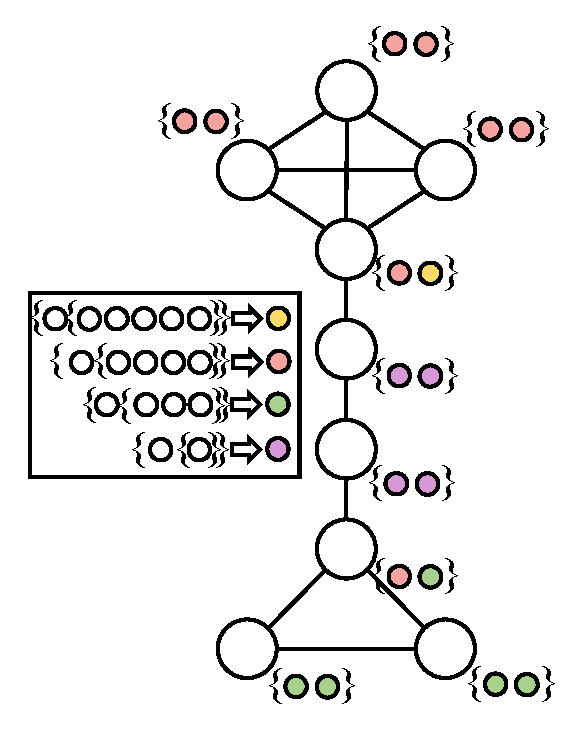
\includegraphics[clip,width=\textwidth]{figures/dfc1_new_new.pdf}
\subcaption{}
\label{subfig:dfc1}
\end{subfigure}%
\hfill
\begin{subfigure}{.245\columnwidth}
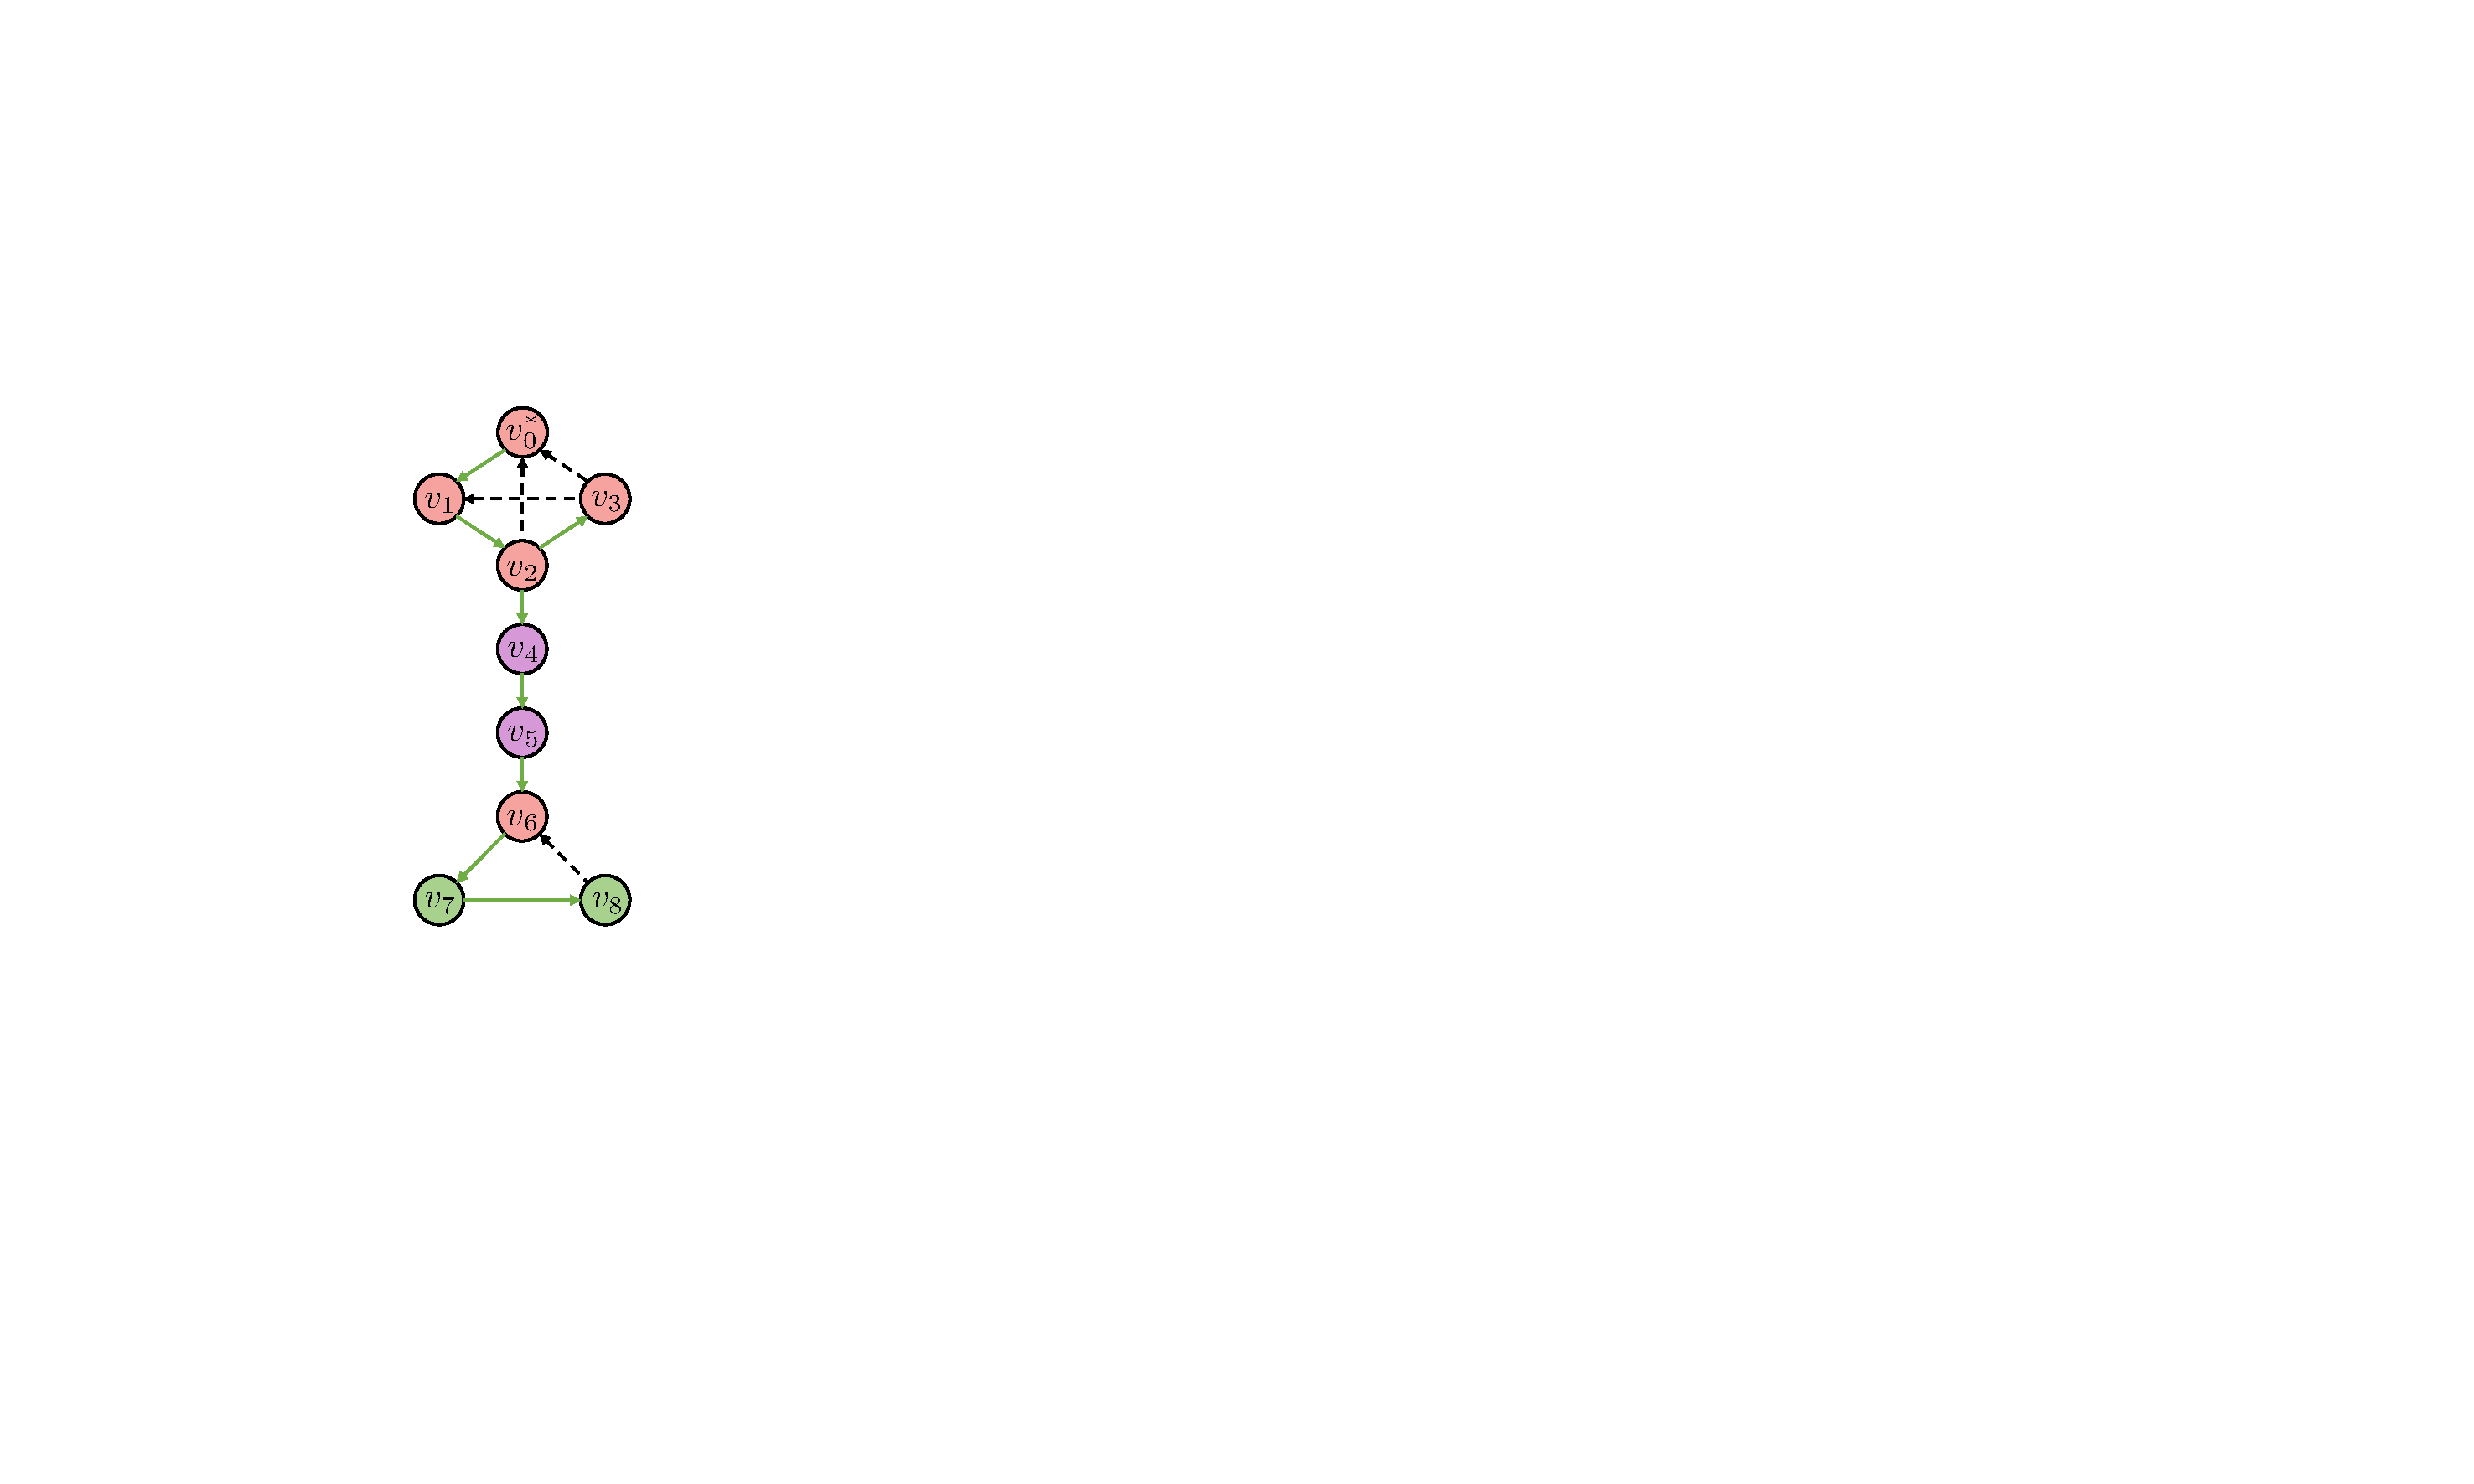
\includegraphics[clip,width=\textwidth]{figures/dfc2_new.pdf}
\subcaption{}
\label{subfig:dfc2}
\end{subfigure}
\hfill
\begin{subfigure}{.245\columnwidth}
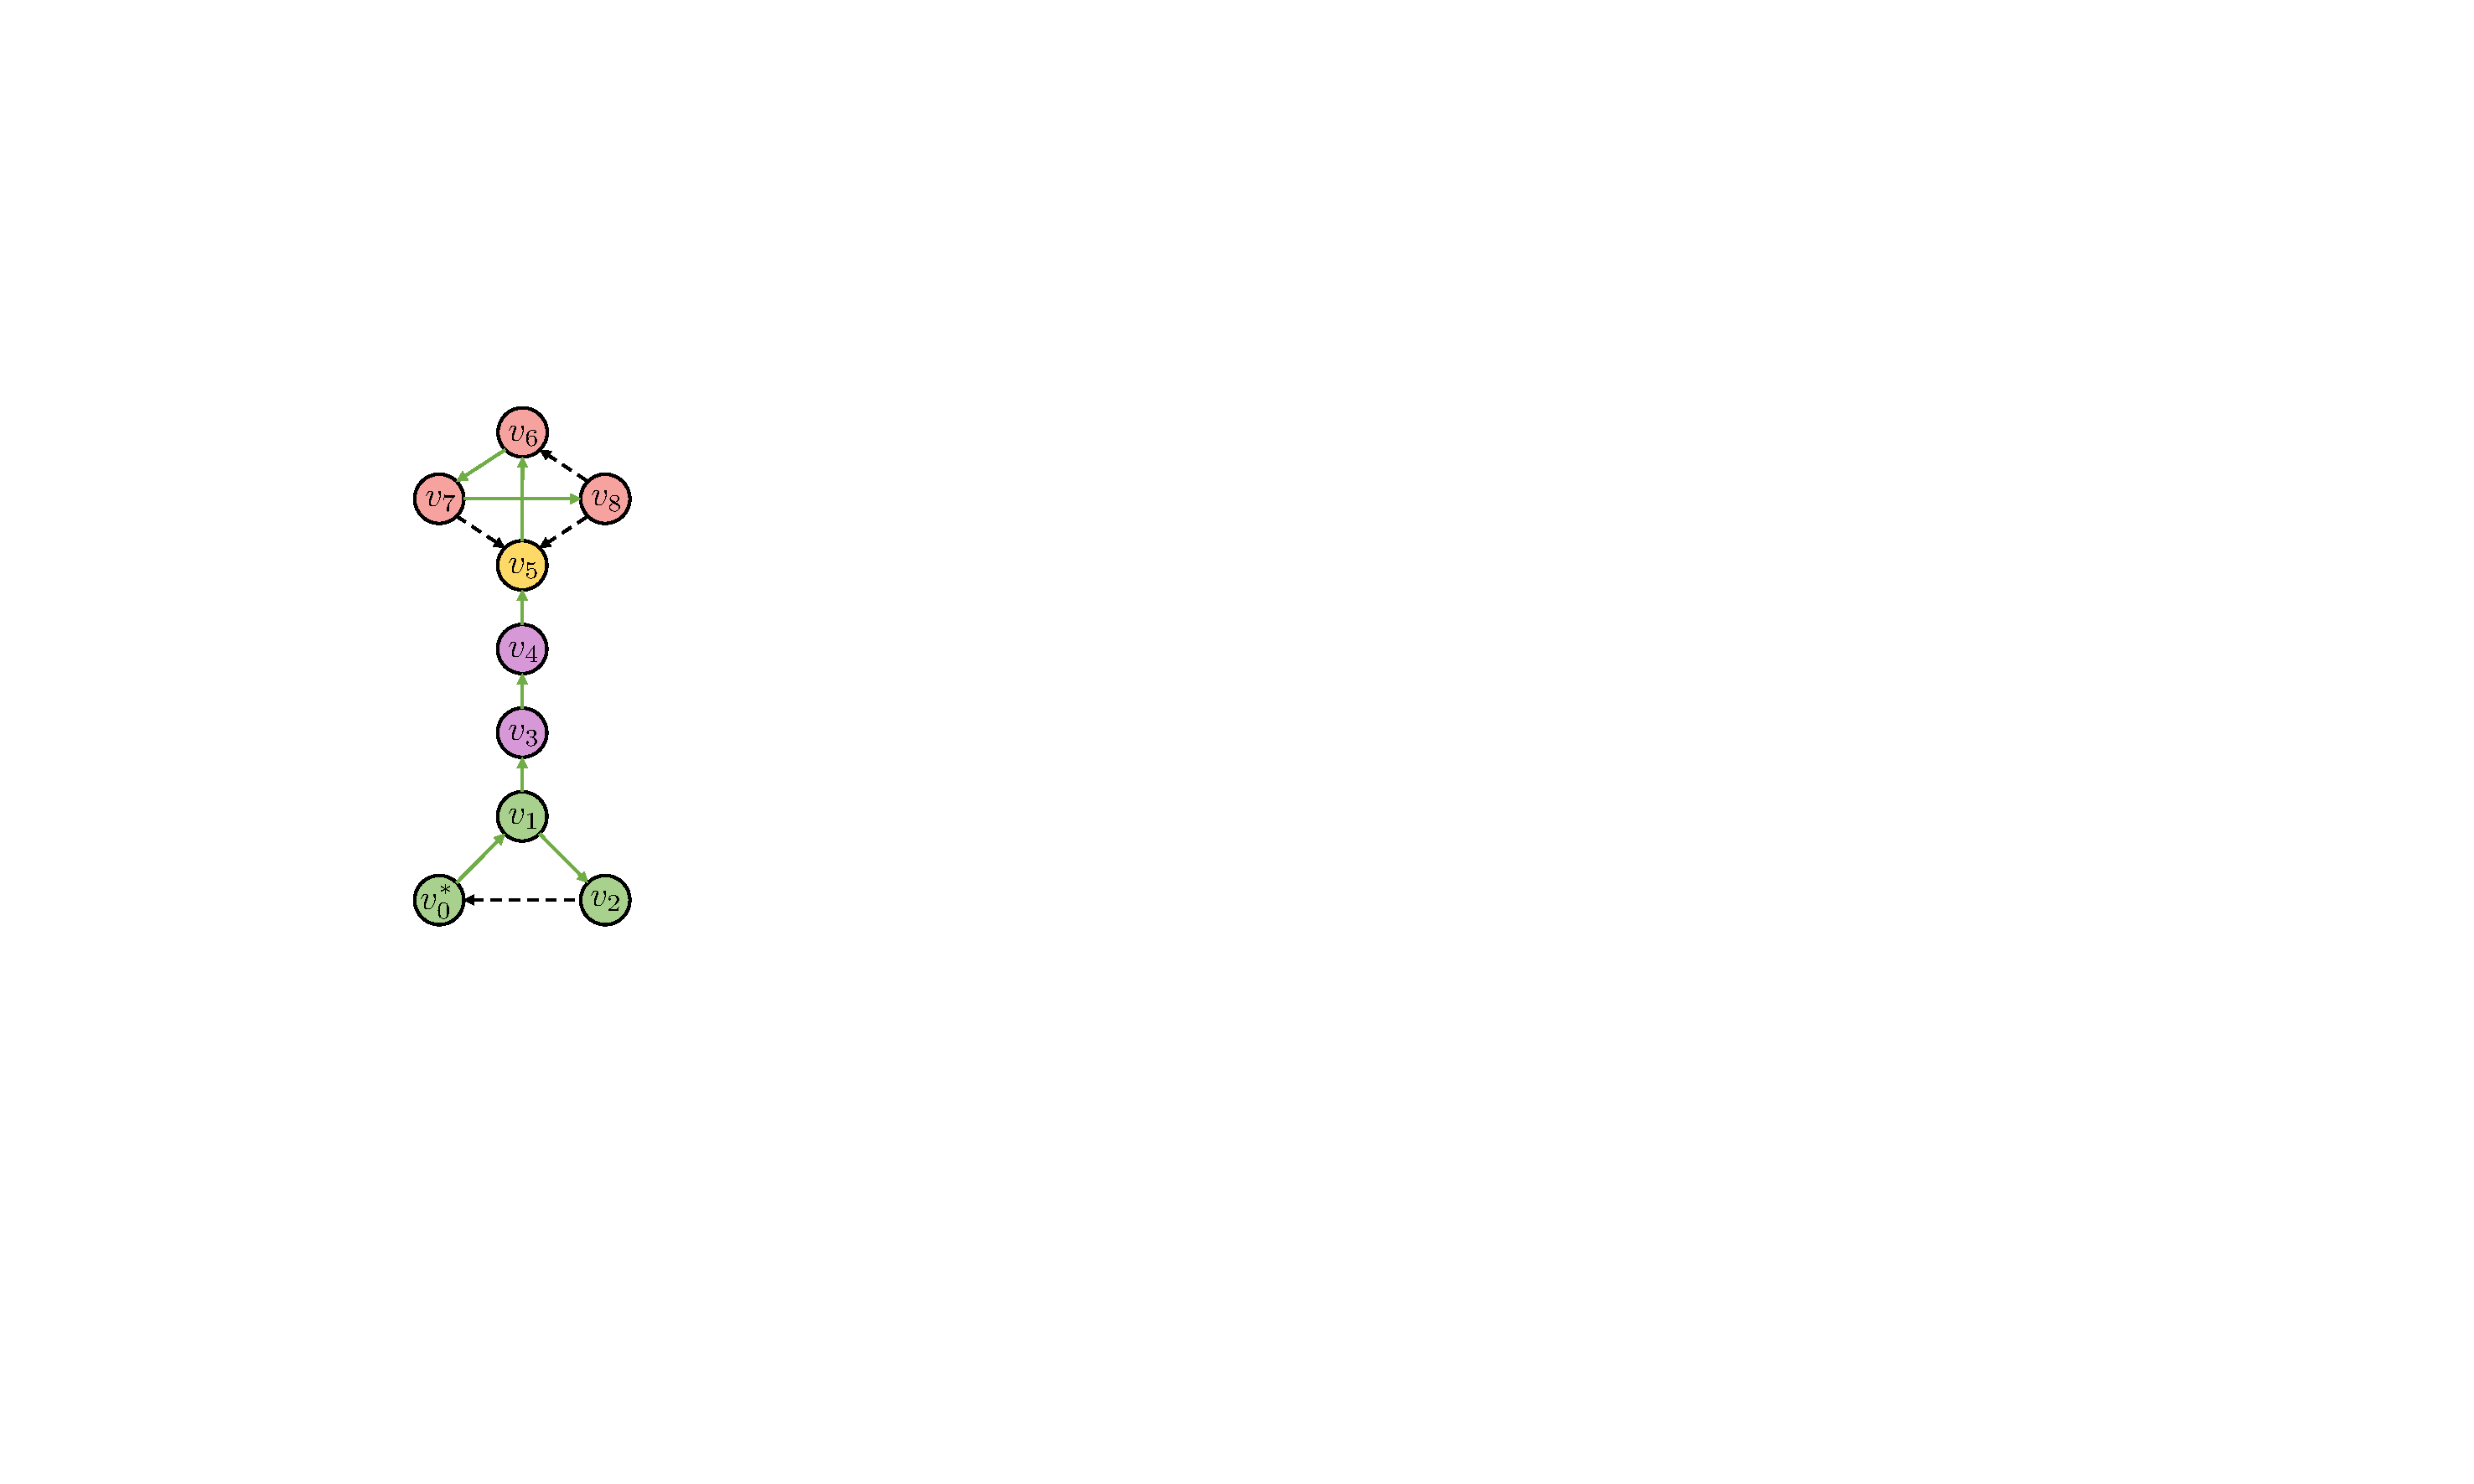
\includegraphics[clip,width=\textwidth]{figures/dfc3_new.pdf}
\subcaption{}
\label{subfig:dfc3}
\end{subfigure}
\caption{
An uneven barbell graph and vertex colours after the first DFC iteration. 
\ref{subfig:dfc1} shows an uncoloured graph, where the vertex colours obtained from \ref{subfig:dfc2} and \ref{subfig:dfc3} are shown next to each vertex.
\ref{subfig:dfc2} and \ref{subfig:dfc3} show DFC with two different roots (marked with *), where each vertex is assigned a new colour by DFC. The colour map is shown on the left.
The subscripted label $v_0$, \dots, $v_5$ denote the visit sequence of each vertex, e.g. $v_1$ is visited after $v_0$.
For brevity, DFC is shown with only two roots.
} 
\label{fig:dfc}
\end{figure}


\paragraph{Depth-first colouring (DFC).} Given a vertex $u\in V$, we define the set of back edges that cover vertex $u$ as
\begin{equation}
\label{eqn:dfc_qu}
    Q_u^{T_v} = \{ \vec{e}:{u \dashv \vec{e}, \vec{e} \in E_{\text{back}}^{T_v}} \}
\end{equation}
We then find all back edges that are transitively crossovered by $Q_u^{T_v}$. We define $D_u^{T_v,0} = Q_u^{T_v}$ for the first iteration. At the $k$-th iteration, we define
\begin{equation*}
    \Delta D_u^{T_v,k} = \{ \vec{e}_2: \vec{e}_1 \nmid \vec{e}_2, \vec{e}_1 \in D_u^{T_v, k-1}, \vec{e}_2 \in E_{\text{back}}^{T_v}  \}
\end{equation*}
\begin{equation*}
    D_u^{T_v,k} := \Delta D_u^{T_v,k}\cup D_u^{T_v, k-1}
\end{equation*}
We use $D_u^{T_v}$ to denote the set of all back edges that are transitively crossovered by edges in $Q_u^{T_v}$, i.e., when the fixed point is reached. The set of vertices covered by at least one back edge in $D_u^{T_v}$ is defined as 
\begin{equation}
\label{eqn:dfs_bu}
    B_u^{T_v} = \{o: o \dashv \vec{e}, \vec{e} \in D^{T_v}_u, o \in V\}.
\end{equation}

We design $\eta$ for DFS, denoted $\eta_{\text{dfc}}$, as
\begin{align}
\label{eqn:sigma_df}
\begin{split}
    \eta_{\text{dfc}}(u, E_{\text{tree}}^{T_v}, &E_{\text{back}}^{T_v}) = \\
    & \{o: (o,u) \in E_{\text{tree}}^{T_v}  \}
    \cup 
    \{o: o \in B_u^{T_v}\}
\end{split}
\end{align}

The part $\{o: (o,u) \in E_{\text{tree}}^{T_v}\}$ preserves vertices that lead to $u$ via tree edges. 
$\{o: o \in B_u^{T_v}\}$ preserves vertices that are covered by the same back edges covering $u$, or by back edges that transitively cover $u$.

The vertex colouring scheme defined using Equations \ref{eqn:lvc-all}, \ref{eqn:lvc}, and \ref{eqn:sigma_df} is called \textit{depth-first colouring} (DFC).
DFC is referred to as DFC-$\delta$ if the search range is limited to a $\delta$-hop neighbourhood for each $u\in V$. Because $\eta_{\text{dfc}}$ is permutation invariant, it is easy to see that DFC-$\delta$ is also permutation invariant.
\cref{fig:dfc} shows an example of colouring an uneven barbell graph using DFC. It can be seen that the vertices at two ends of the barbell share the same colour, while the vertices on the connecting path have different colours.
\begin{restatable}[]{lemma}{dfcinvariance}
\label{lemma:dfcinvariance}
$\eta_{\text{dfc}}$ is invariant under search order permutation.
\end{restatable}


% When visiting $u$, we identify the back edges starting from $u$ and subsequently a set of vertices $\mathbb{S}_u$ these back edges pointing to. Then by inspecting the search path leads from $v$ to $u$, we can identify the set of vertices that are on the same cycles as $u$, denoted as $\mathbb{D}_u$. We then colour these vertices accordingly.

% \begin{align}
%     \mathbb{S}_u = & \{ o:{(u, o) \in E_{\text{back}}} \}  \\
%     \mathbb{D}_{u} = & \bigcup_{o\in \mathbb{S}_u} \{w \in \mathcal{P}_{ou}:  \mathcal{P}_{ou} \vartriangleleft \mathcal{P}_{vu}\}
% \end{align}

% \begin{align}
% \label{eqn:dfs_lvc_forward}
% \forall w \in & \mathbb{D}_u \text{ do}: \text{(DFS forward-update)} \nonumber\\
% & \lambda_v(w):= \phi\Bigl(\lambda(w), \psi\bigl(\{\!\!\{\lambda_v(o): o \in \mathbb{D}_u\}\!\!\}\bigr)\Bigr)
% \end{align}
% We call this the \textit{DFS forward-update}. The vertex $w$ is assigned an updated colour based on the its current colour and the multiset of current colours from vertices in the same cycle(s). This ensures the the assigned colours are invariant to permutation: regardless of which branch DFS chooses to explore first, vertices on the same cycles(s) have their colour updated the same way. This also aligns with Tarjan's algorithm where vertices form a cycle share the same low value.

% Now we look at \textit{DFS backward-update}. After the forward-update, we have all cycles coloured. However, we are missing the information about visiting sequence. To incorporate it, we can colour the vertices not in the same cycles recursively according to their visiting order. For each vertex $u$, we first find its parent which is not in the same cycle(s) with $u$.
% \begin{align}
% \mathbb{C} = &\{ \mathcal{P}_{ab}:\mathcal{P}_{ab}\triangleleft \mathcal{P}\in \mathbb{P}_v \land (b,a) \in E_{\text{back}} \}\\
% \mathbb{W}_u = &\{w: (w, u) \in E_{\text{tree}}\land (w, u) \notin \mathcal{P} \in \mathbb{C}\}
% \end{align}
% $\mathbb{C}$ is a search path set where each path participates in at least one cycle. $\mathbb{W}$ contains $w$, the parent of $u$, if $(w,u)$ does not participate in any cycle, otherwise $\mathbb{W}$ is empty.

% \begin{align}
% \label{eqn:dfs_lvc_backward}
%  \forall u \in & V \text{ by visiting order do}: \text{(DFS backward-update)} \nonumber\\
% & \lambda_v(u):= \phi\Bigl(\lambda_v(u), \psi\bigl(\{\!\!\{\lambda_v(w): w \in \mathbb{W}_u\}\!\!\}\bigr)\Bigr)
% \end{align}
% We name the DFS-guided LVC using \cref{eqn:dfs_lvc_forward,eqn:dfs_lvc_backward} as LVC-DFS.

% \q{(General comments: we need to meet and discuss this. In the current form, it doesn't look completely clear to me. But I feel you're generally on the right track of making progresses. Indeed, very well done for the progress you have made!)}

\paragraph{Distinguishing biconnectivity.}
We hereby show that DFC is expressive for distinguishing graphs that exhibit the biconnectivity property. %described by \citet{anonymous2023rethinking}.
Graph biconnectivity is a well-studied topic in graph theory and often discussed in the context of network flow and planar graph isomorphism~\citep{Hopcroft1973-lu}. \citet{anonymous2023rethinking} first draw attention to biconnectivity in the context of GNN and show that most GNNs cannot learn biconnectivity. 
% A biconnected component of a graph is a connected subgraph that cannot be disconnected by deleting any single node. 

A vertex $v\in V$ is said to be a \emph{cut vertex} (or \emph{articulation point}) in $G$ if removing the vertex disconnects $G$. Thus, the removal of a cut vertex increases the number of connected components in a graph (a connected component is an inducted subgraph of $G$ in which each pair of vertices is connected via a path). Similarly, an edge $(v,u)\in E$ is a \emph{cut edge} (or \emph{bridge}) if removing $(v,u)$ increases the number of connected components. A graph is \emph{vertex-biconnected} if it is connected and does not have any cut vertices. Similarly, A graph is \emph{edge-biconnected} if it is connected and does not have any cut edges.

%We show that DFC is expressive for distinguishing graphs that exhibit the properties below.

\begin{restatable}[]{lemma}{dfcbiconnectivity}
\label{lemma:dfcbiconnectivity}
Let $G$ and $H$ be two graphs, and %\q{$\lambda^{*}(v)$ be the stable colour of a vertex $v$ after $j$ colouring iterations.} So
$\{\!\!\{ \lambda(u):u\in V_G\}\!\!\}$ and $\{\!\!\{ \lambda(u'):u'\in V_H\}\!\!\}$ be the corresponding multisets of stable vertex colours of $G$ and $H$ by running DFC. Then the following statements hold: 


\begin{itemize}
    \item For any two vertices $u\in V_G$ and $u'\in V_H$, if $\lambda(u) = \lambda(u')$, then $u$ is a cut vertex if and only if $u'$ is a cut vertex.
    \item For any two edges $(u_1,u_2)\in E_G$ and $(u'_1,u'_2)\in E_H$, if $\{\!\!\{ \lambda(u_1), \lambda(u_2)\}\!\!\} = \{\!\!\{ \lambda(u'_1), \lambda(u'_2)\}\!\!\}$, then $(u_1,u_2)$ is a cut edge if and only if $(u'_1,u'_2)$ is a cut edge.
    \item If $G$ is vertex/edge-biconnected but $H$ is not, then $\{\!\!\{\lambda(u): u\in V_G\}\!\!\} \neq \{\!\!\{\lambda(u'):u'\in V_H\}\!\!\}$.
    % \item If $\{\!\!\{\lambda_G(v):v\in V_G\}\!\!\} = \{\!\!\{\lambda_H(u):u\in V_H\}\!\!\}$, then $\operatorname{BCETree}(G)\simeq \operatorname{BCETree}(H)$ (\s{Pending proof})
\end{itemize}
\end{restatable}

% \s{\citet{anonymous2023rethinking} haven't release dataset for biconnectivity yet}

\begin{restatable}[]{corollary}{vertexinbiconnectedcomponent}
\label{corollary:vertexinbiconnectedcomponent}
Let $u\in V_G$ and $u'\in V_H$ be two vertices, and $\lambda(u) = \lambda(u')$. Then $u$ is in a cycle if and only if $u'$ is in a cycle. 

%\q{(notes from Qing: it would need some changes if the notation for stable colour is changed.)}
\end{restatable}

% \begin{definition}(Distance-Incremental Search)
% \label{def:dit}
% $\mathcal{T}$ is a distance-incremental search (DIS) if 
% \begin{itemize}
%     \item If $v$ and $u$ are connected in $N_{\delta}(v)$ for any $\delta > t > 0$, $\mathcal{T}$ always return the same $\mathcal{P}_{vu}$ by searching $N_{\delta}(v)$.
%     \item Given $\delta \geq 0$, vertices $\{w\in V: d_{vw}\leq \delta\}$ are visited before visiting $\{u\in V : d_{vu} \geq \delta\}$.
% \end{itemize}
% \end{definition}

% \begin{restatable}[]{lemma}{pathsets}
% \label{lemma:path_sets}
% Let $\mathbb{P}_{v,\delta}=\{\mathcal{P}_{vu}: u\in N_\delta(v)\}$ be a set of paths found by a DIS rooted at $v$. We have $\mathbb{P}_{v,\delta} \subseteq \mathbb{P}_{v,\delta+1}$. Also for every $\mathcal{P}\in \mathbb{P}_{v,\delta+1}$, there is a path $\mathcal{P}'\in \mathbb{P}_{v,\delta}$ so that  $\mathcal{P}'\subseteq \mathcal{P}$.
% \begin{itemize}
%     \item For any path $\mathcal{P}_{vu_1} \in \mathbb{P}_{v,\delta}$, there exists a path $\mathcal{P}_{vu_2} \in \mathbb{P}_{v,\delta+1}$ so that $\mathcal{P}_{vu_1}\subseteq \mathcal{P}_{vu_1}$;
%     \item  For any path $\mathcal{P}_{vu_1} \in \mathbb{P}_{v,\delta+1}$, there exists a path $\mathcal{P}_{vu_2} \in \mathbb{P}_{v,\delta}$ so that $\mathcal{P}_{vu_1}\supseteq \mathcal{P}_{vu_2}$;
%     \item  $\mathbb{P}_{v,\delta} \subseteq \mathbb{P}_{v,\delta+1}$
% \end{itemize}
% \end{restatable}

\subsection{Expressivity Analysis}

\paragraph{Comparison with 1-WL.}
When $\delta=1$, it is easy to see that search trees in BFC contain only direct neighbours of the root and edges between the root and its neighbours, and there are no back edges. Thus, we have the lemma below.
\begin{restatable}[]{lemma}{onewlequal}
\label{lemma:1wlequal}
BFC-1 is equivalent to 1-WL.
\end{restatable}

When $\delta=1$, search trees in DFC contain direct neighbours of the root, edges between the root and the neighbours, and edges between the neighbours. We have the following lemma.
\begin{restatable}[]{lemma}{dfconewl}
\label{lemma:dfc1wl}
DFC-1 is more expressive than 1-WL.
\end{restatable}


\begin{restatable}[]{corollary}{bfcdistinguish}
\label{lemma:bfc_distinguish}
When $\delta > 1$, BFC-$\delta$ can distinguish one or more pairs of graphs that cannot be distinguished by 1-WL.
\end{restatable}

\begin{restatable}[]{corollary}{dfcdistinguish}
\label{lemma:dfc_distinguish}
When $\delta\geq 1$, DFC-$\delta$ can distinguish one or more pairs of graphs that cannot be distinguished by 1-WL.
\end{restatable}


Taking a pair of graphs - one is two triangles and the other is one six-cycle - for example, these two graphs cannot be distinguished by 1-WL. However, they can be distinguished by BFC-2 and DFC-1 (\cref{fig:circle_examples}).

\begin{figure}[h]
\centering
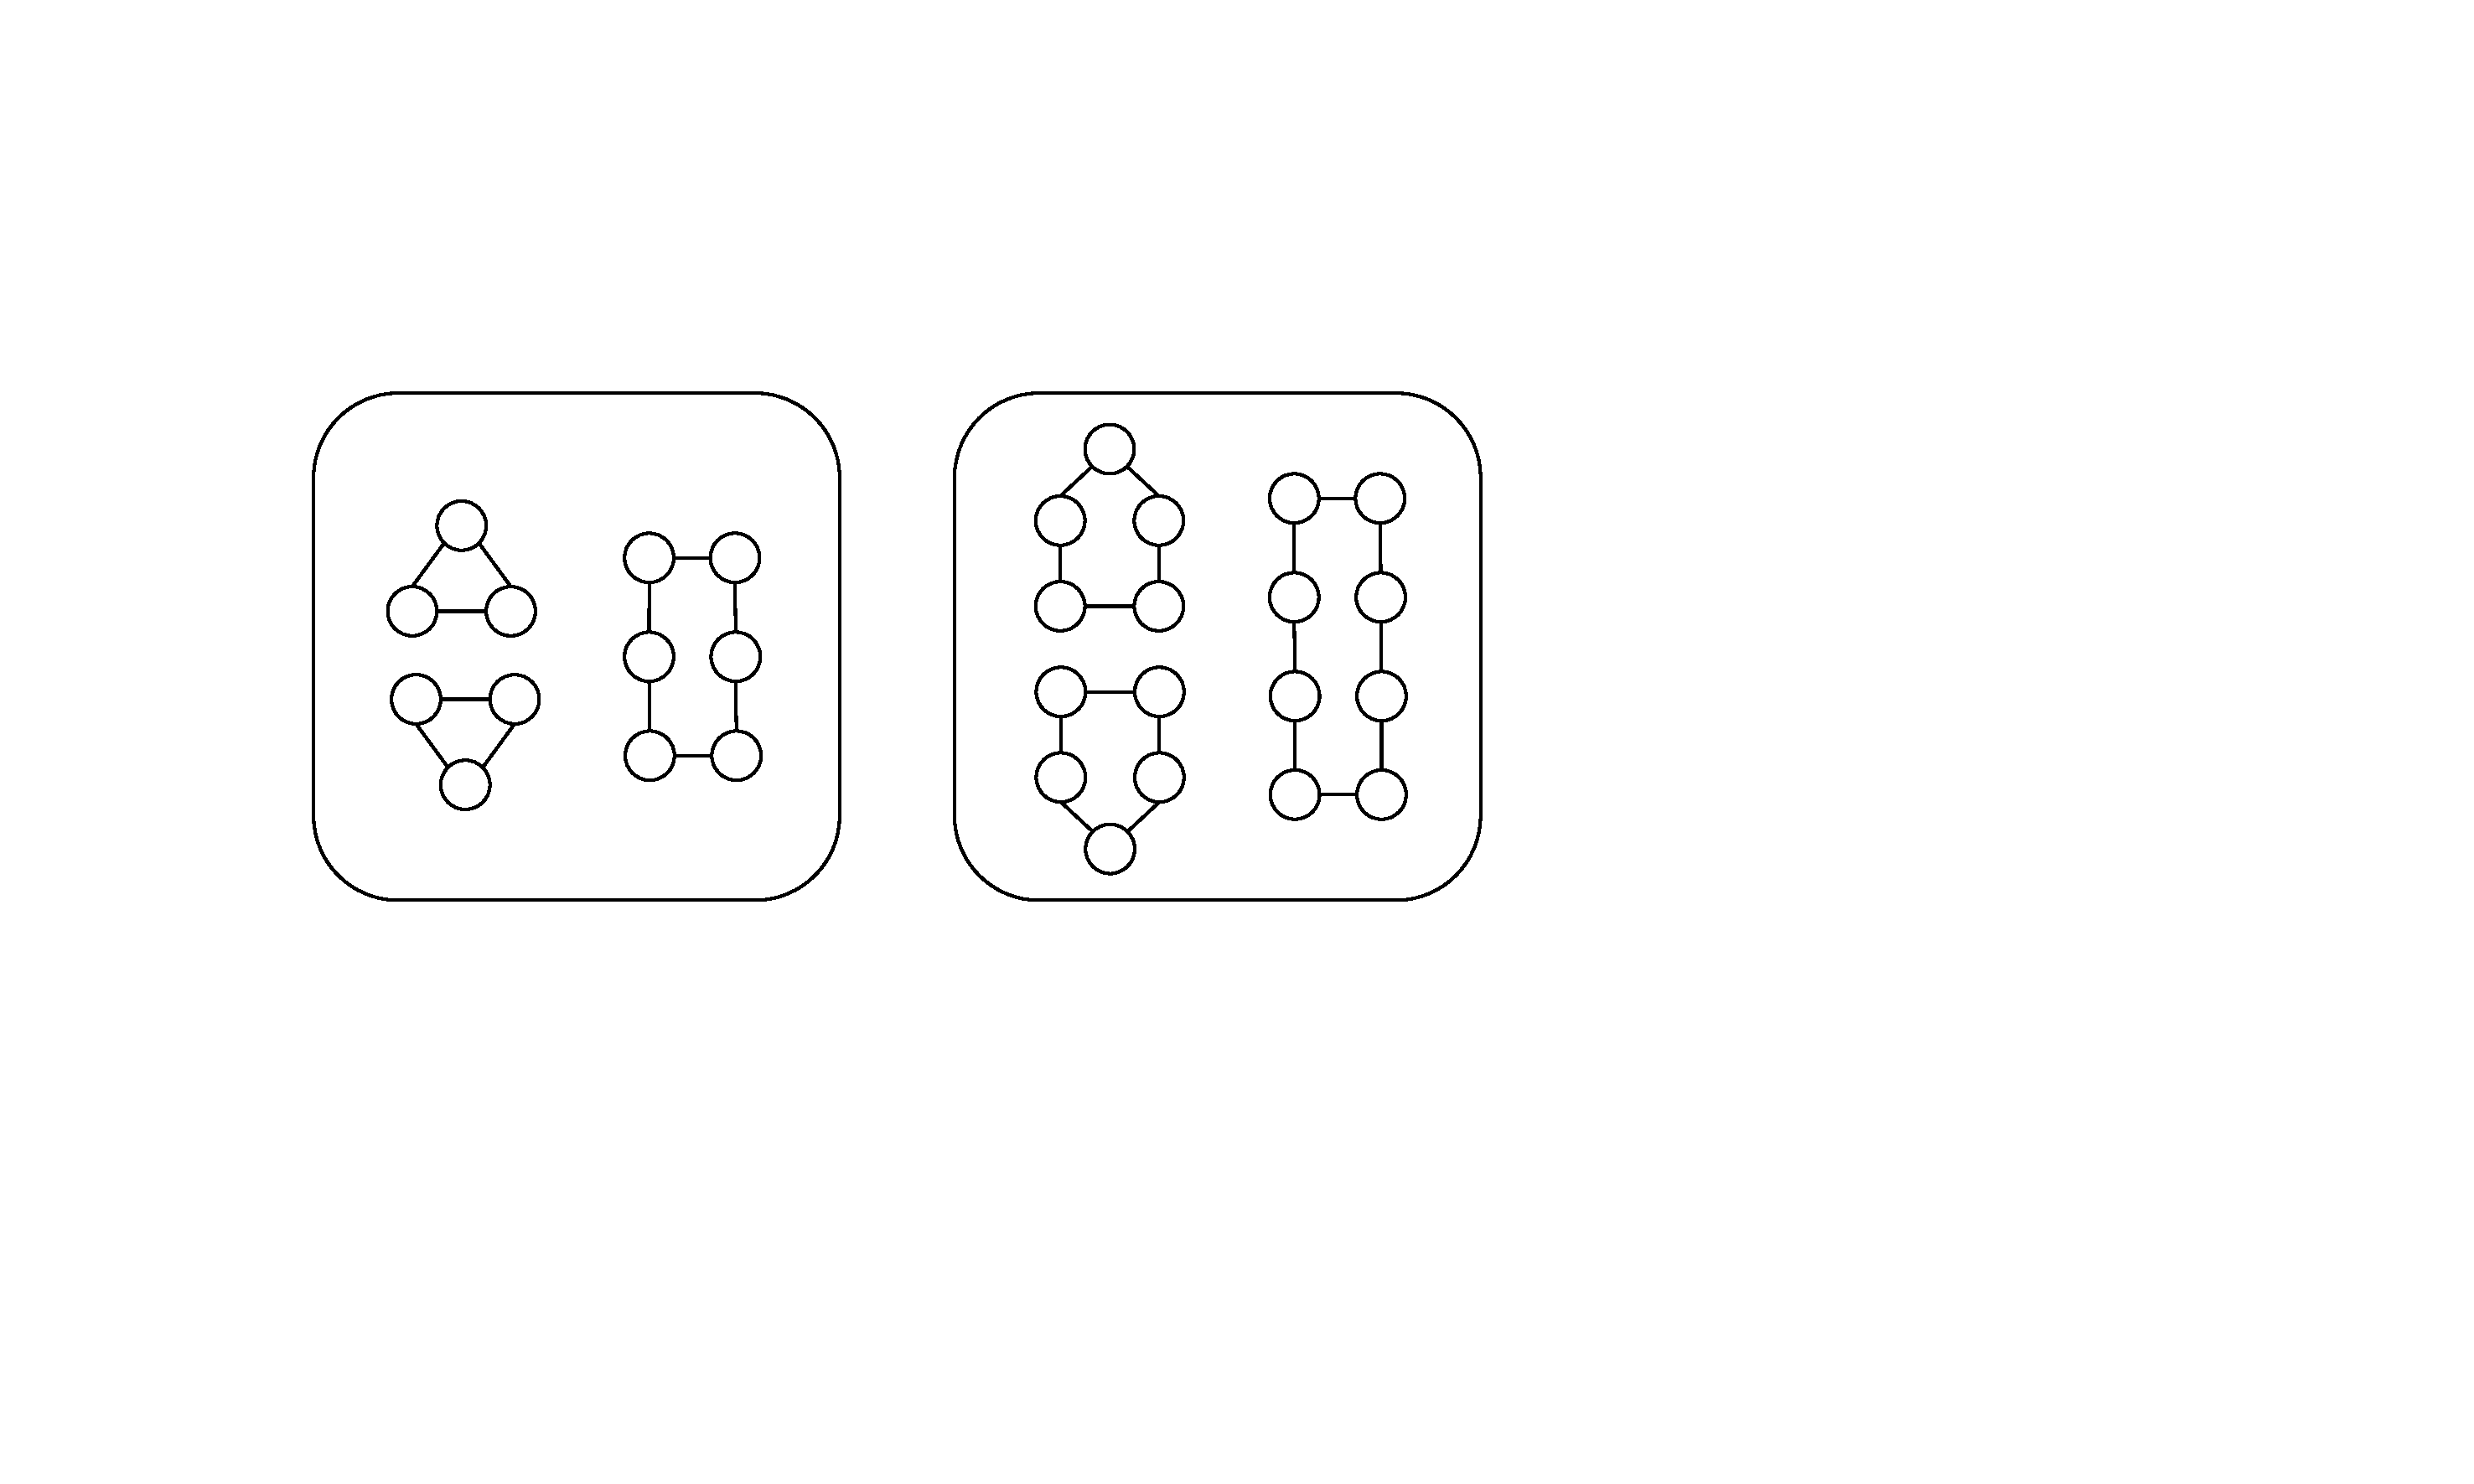
\includegraphics[clip,width=0.75\columnwidth]{figures/circle_example_new.pdf}
\caption{(Left) A graph pair can be distinguished by BFC-2 and DFC-1 but not by BFC-1 and 1-WL. (Right)  A graph pair can be distinguished by BFC-3 and DFC-2 but not by BFC-2, DFC-1 and 1-WL.}
\label{fig:circle_examples}
\end{figure}


%A comparison of the stable colourings obtained by executing the algorithm on each of two given graphs can often be used to prove their non-isomorphism.

% \begin{restatable}[]{lemma}{expressityequal}
% \label{lemma:expressity_equal}
% When a search algorithm that satisfies \autoref{def:dit} is used, $LVC^{\delta+1}$ is at least as expressive as $LVC^{\delta}$ in distinguishing non-isomorphic graphs.
% \end{restatable}

\paragraph{Comparison with 3-WL.}
We can also show that, regardless of the choice of $\delta$, BFC is no more expressive than 3-WL. This leads to the following theorem.

\begin{restatable}[]{thm}{bfcthreewl}
\label{thm:bfc3wl}
The expressive power of BFC-$\delta$ is strictly upper bounded by 3-WL.
\end{restatable}

However, unlike BFS, DFC can distinguish graphs that cannot be distinguished by 3-WL. For example, DFC-1 can distinguish the strongly regular graph pair shown in \cref{fig:rook_shrikhande} which cannot be distinguished by 3-WL: the 4x4 Rook's graph of 16 vertices~\citep{Wagon_Weisstein} and the Shrikhande graph~\citep{Shrikhande_graph}. In the 4x4 Rook's graph, each vertex's 1-hop subgraph has a cut vertex, while there is no cut vertex in the Shrikhande graph. So according to \cref{lemma:dfcbiconnectivity}, DFC-1 can distinguish these two graphs. On the other hand, there are also graphs that 3-WL can distinguish but DFC-1 cannot. For example, the right graph pair in \cref{fig:circle_examples}. Thus, we have the following theorem.

\begin{restatable}[]{thm}{dfcthreewl}
\label{thm:dfc3wl}
The expressive powers of DFC-$\delta$ and 3-WL are incomparable.
\end{restatable}


\begin{figure}[h]
\centering
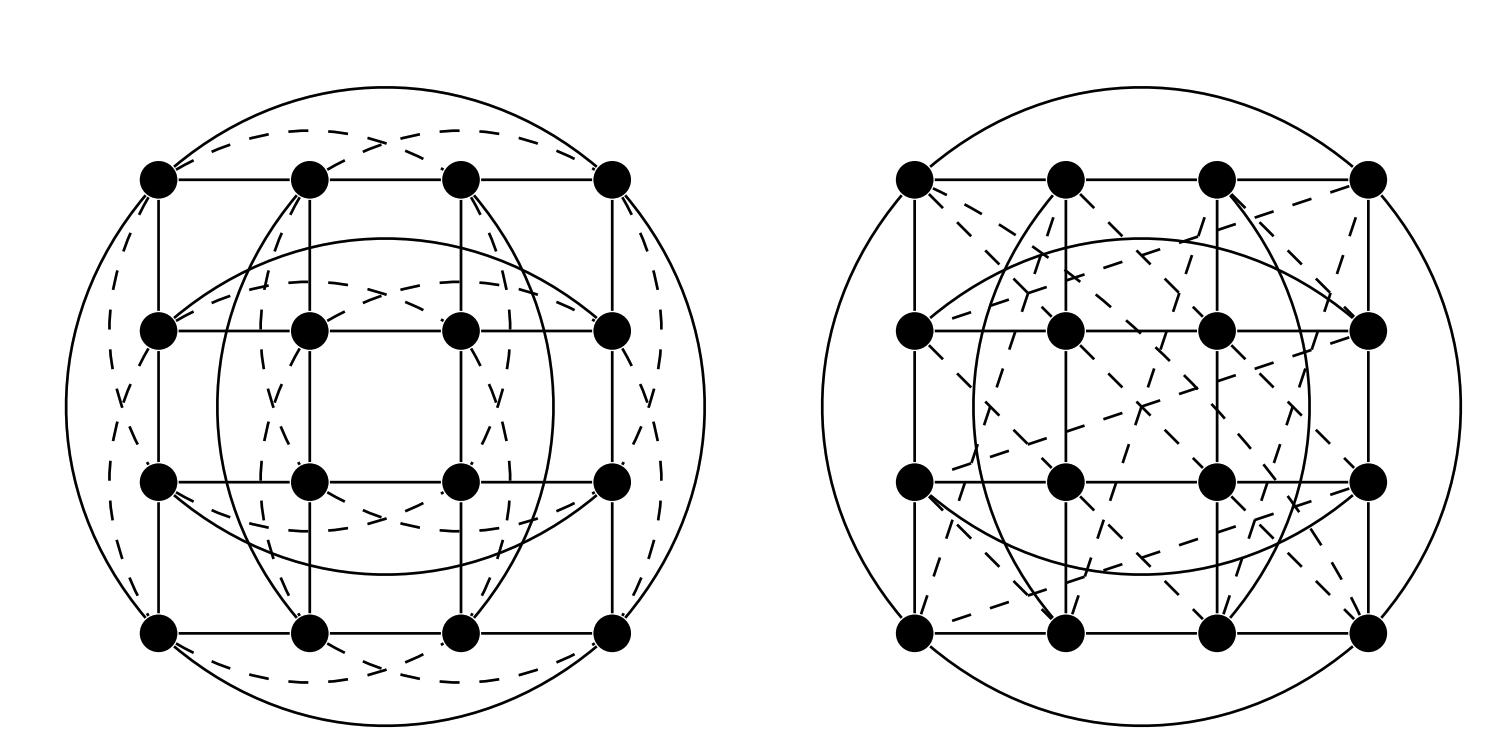
\includegraphics[clip,width=0.75\columnwidth]{figures/Shrikhande_Rook_graph.png}
\caption{The 4x4 Rook’s graph and the Shrikhande graph \citet{ARVIND202042}. Some edges are dashed for readability.}
\label{fig:rook_shrikhande}
\end{figure}

\paragraph{Expressivity hierarchy.} The following theorem states that there exists a hierarchy among the expressive powers of BFC-$\delta$ when increasing $\delta$.

\begin{restatable}[]{thm}{bfcexpressitybeyond}
\label{thm:bfcexpressitybeyond}
BFC-$\delta$+1 is strictly more expressive than BFC-$\delta$ in distinguishing non-isomorphic graphs.
\end{restatable}

\cref{thm:bfcexpressitybeyond} implies that BFC can be used as an alternative way, separating from the WL test hierarchy, to measure the expressivity of GNNs. 

Nevertheless, DFC-$\delta$ does not exhibit a hierarchy. \cref{fig:dfc_expressity_delta} 
depicts two pairs of non-isomorphic graph pairs: one pair can be distinguished by DFC-1 but not by DFC-2 while the other pair can be distinguished by DFC-2 but not by DFC-3. This leads to Theorem~\ref{thm:dfcexpressitynotbeyond} below. 

\begin{restatable}[]{thm}{dfcexpressitynotbeyond}
\label{thm:dfcexpressitynotbeyond}
DFC-$\delta$+1 is not necessarily more expressive than DFC-$\delta$ in distinguishing non-isomorphic graphs. 
\end{restatable}

 

\begin{figure}[ht]
\centering
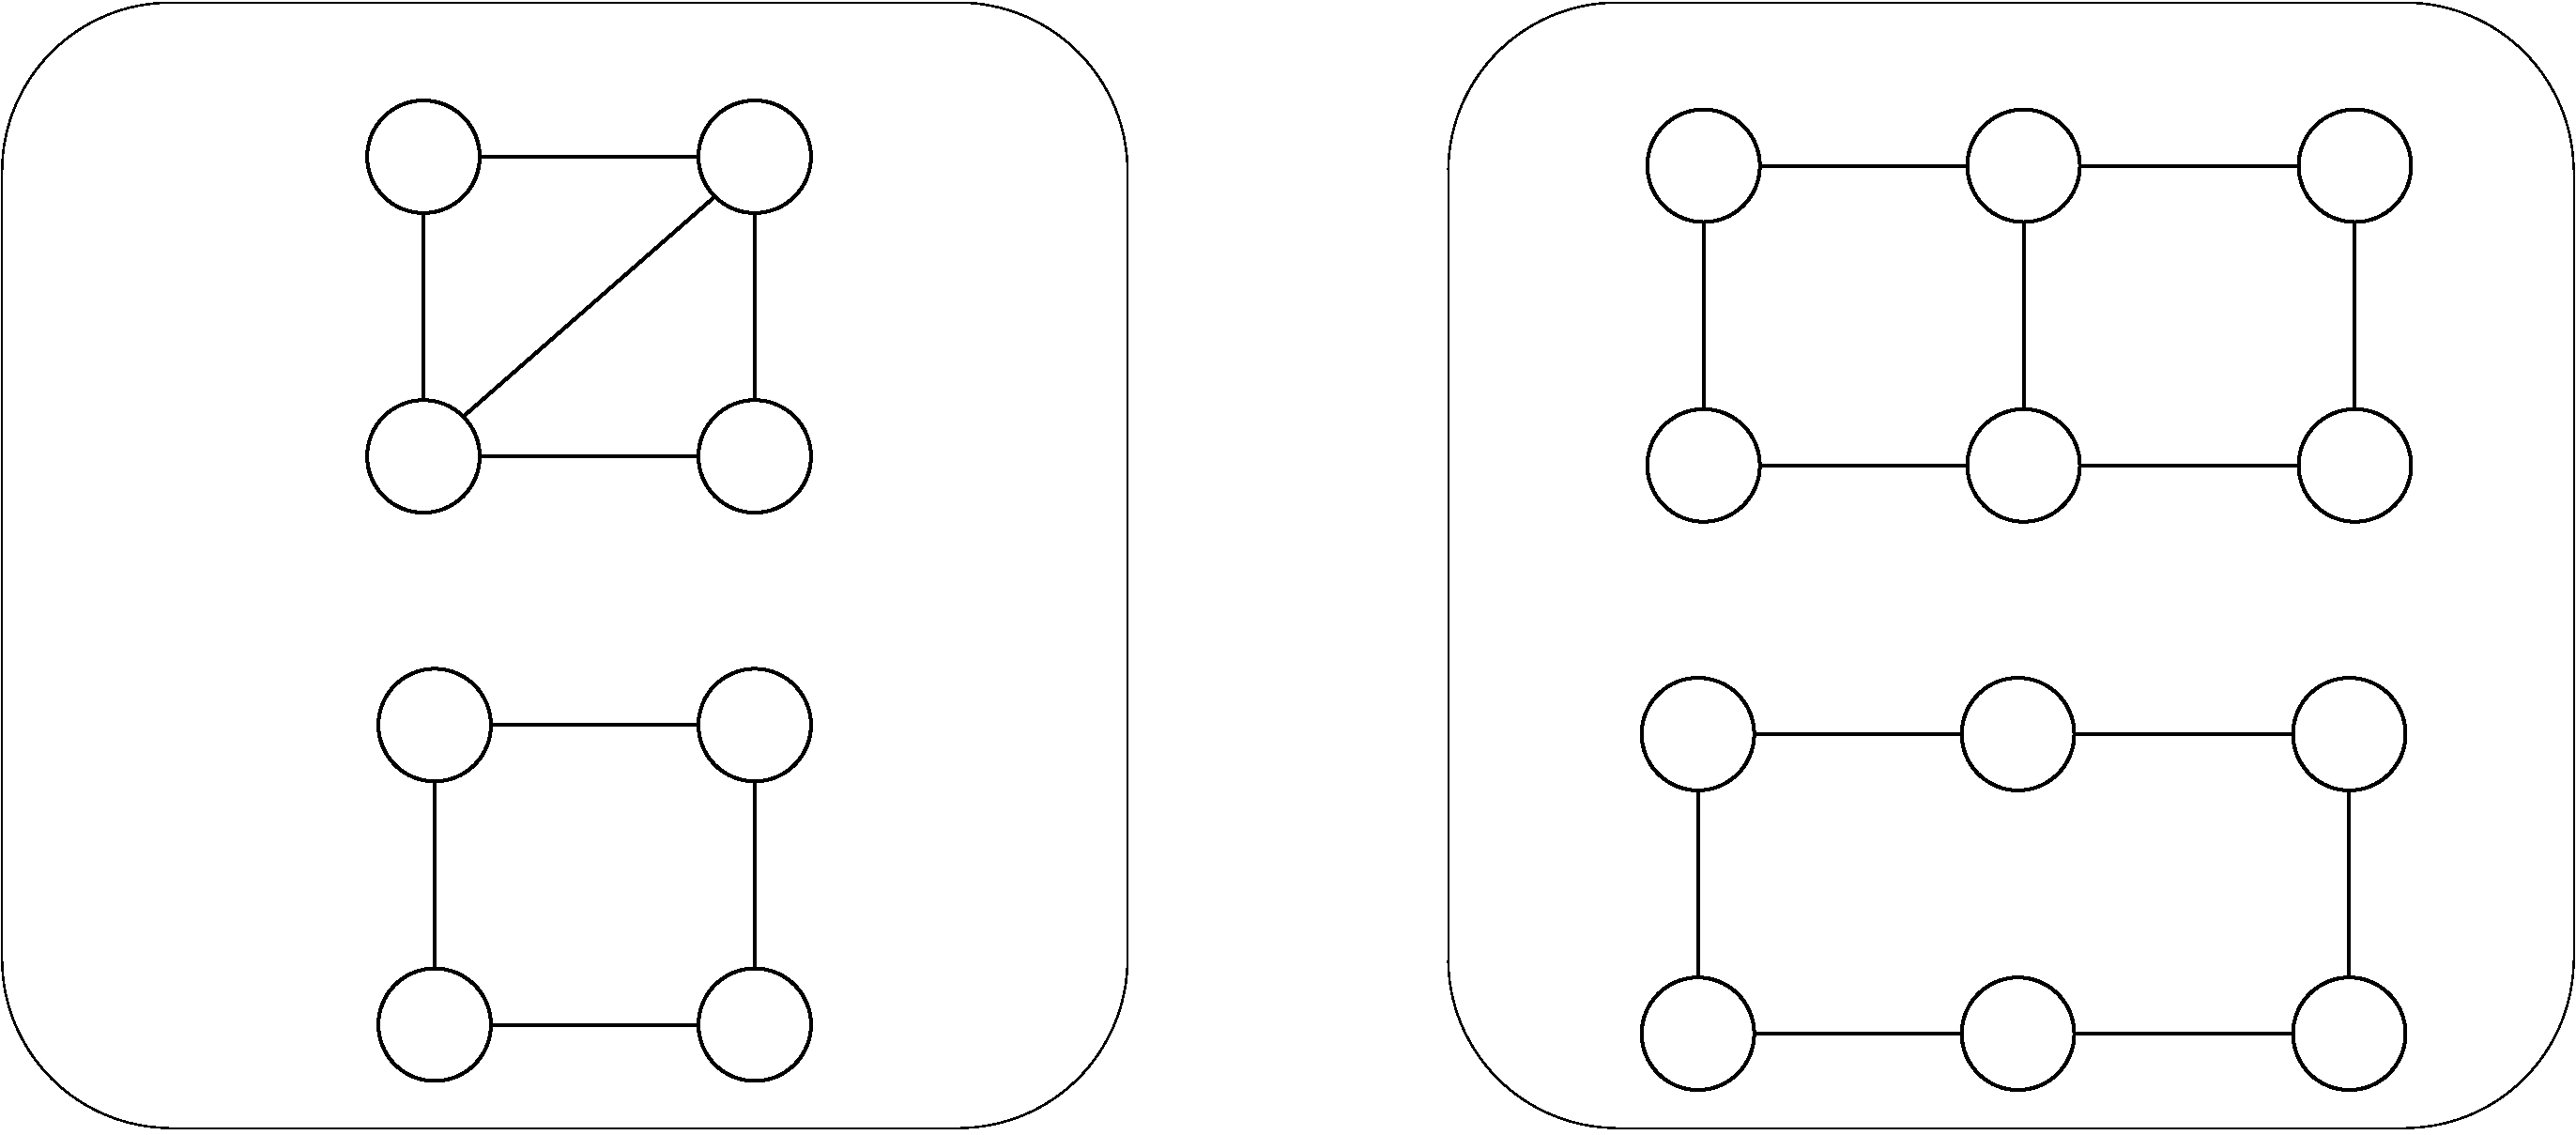
\includegraphics[clip,width=0.65\columnwidth]{figures/dfc_expressity_delta_1_2_new.pdf}
\caption{Non-isomorphic graph pairs. A pair can be distinguished by DFC-1 but not by DFC-2 (Left). A pair can be distinguished by DFC-2 but not by DFC-3 (Right).} 
\label{fig:dfc_expressity_delta}
\end{figure}


% \subsection{D-LVC Expressivity Hierarchy}

% In some cases, one might prefer to use a traversal approach that doesn't satisfy \autoref{def:dit}. For example, one might use run random walk multiple times rooted at vertex $v$ until all vertices in $N_{\delta}(v)$ are visited, for the sake of capturing network flow. In such cases, a similar hierarchy can be obtained by using a modified colour update rule:
% \begin{equation}
% \label{eqn:lvc}
%     \lambda_v(u):= \texttt{hash}(\lambda(u), \q{\eta(v, u),} \{\!\!\{\lambda_v(w)|(u,w)\in E \text{ and }  w\in N_{visited}(v)\}\!\!\})
% \end{equation}

% where $\eta(v, u)$ encodes the distance information between $v$ and $u$, e.g. shortest distance or resistance distance. We denote this colouring algorithm as D-LVC.

% \begin{restatable}[]{thm}{expressitybeyonddlvc}
% \label{thm:expressitybeyonddlvc}
%  $\text{D-LVC}^{\delta+1}$ is strictly more expressive than $\text{D-LVC}^{\delta}$ in distinguishing non-isomorphic graphs.
% \end{restatable}

% It is easy to see \autoref{lemma:1wl_expressity} and \autoref{lemma:lvc_distinguish} also hold for D-LVC




% \section{Extension}
% The rules to update $N_{visited}$ in \autoref{eqn:lvc} can be extended to any graph traversal algorithms beyond BFS.\autoref{lemma:1wl_expressity}, \autoref{lemma:expressity_equal} and \autoref{thm:expressity_beyond} 
% hold for any graph traversal algorithms that, starts with a vertex $u$, parameterised with depth $\delta$, and satisfy the following two properties.
% \begin{itemize}
%     \item when $\delta=1$, $N_{\delta}(u) = \{u\}$.
%     \item when $\delta>1$, $P_{\delta}(u) \subseteq P_{\delta+1}(u)$
% \end{itemize}
% where $P_{\delta}(u)$ is a set of vertex sequences, each sequence is a path that ends at $u$ and starts at a vertex that is $\delta$ steps away from $u$. For instance, BFS variants, like best-first search, $A^*$ search, satisfies above. DFS, on the other hand, does not satisfy property 2. Because when $\delta$ increments, it is possible to discover a new path using DFS, $p_1$, of length $\delta+1$ connects $u$ and a vertex that $v$ is $\delta$ steps away. Because each vertex is visited only once, the discovery of $p_1$ removes a length-$\delta$ path $p_2$ that connects $v$ and $u$ in $P_{\delta}(u)$.
% Denote such traversal algorithms as $\mathcal{T}$, we have

% \begin{restatable}[]{thm}{onewlexpressityt}
% \label{thm:1wl_expressity_t}
% $LVC_{\mathcal{T}}$ with $\delta=1$ is equivalent to 1-WL in distinguishing non-isomorphic graphs.
% \end{restatable}

% \begin{restatable}[]{thm}{expressitybeyondt}
% \label{thm:expressity_beyond_t}
% $LVC_{\mathcal{T}}^{\delta+1}$ is strictly more expressive than $LVC_{\mathcal{T}}^{\delta}$ in distinguishing non-isomorphic graphs.
% \end{restatable}

% This opens door for creating variants of this algorithm with guaranteed expressiveness. For instance, one may combine $A^*$ and Beam Search to develop an new algorithm such as \autoref{alg:a_star}.

% \begin{algorithm}[th]
% \caption{LVC}\label{alg:lvc}
% \begin{algorithmic}[1]
% \STATE {\bfseries Input:} Graph $G = (V, E)$, search radius $\delta$, initial vertex colour $\lambda$
% \STATE {\bfseries Output:} Updated vertex colour $\lambda$

% \FOR{$v \in V$}
% \STATE Initialize $\lambda_v \gets \lambda$
% \STATE $\text{search\_and\_colour}(G, v, v, \delta, \lambda, \lambda_v)$
% \ENDFOR

% \FOR{$u \in V$}
% \STATE $\lambda(u):= \texttt{hash}(\lambda(u), \{\!\!\{\lambda_v(u)| v\in N_{\delta}(u)\}\!\!\})$
% \ENDFOR

% \end{algorithmic}
% \end{algorithm}

% \begin{algorithm}[th]
% \caption{$\text{search\_and\_colour}(G, v, w, \delta, \lambda, \lambda_v(w))$}
% \label{alg:search_and_colour}
% \begin{algorithmic}[1]
% \STATE {\bfseries Input:} Graph $G$, root vertex $v$, current vertex $w$, search radius $\delta$, vertex colour $\lambda$, vertex colour $\lambda_v$, 
% \STATE {\bfseries Output:} Updated vertex colour $\lambda_v$
% \STATE $u \gets \text{next}(G, w)$
% \IF{$d_{vu}\leq \delta$}
% \STATE $\lambda_v(u) \gets \texttt{hash}(\lambda(u), \lambda_v(w))$
% \STATE $\text{search\_and\_colour}(G, v, u, \delta, \lambda, \lambda_v)$
% \ENDIF
% \end{algorithmic}
% \end{algorithm}


